\chapter{基于模型的方法计算$\CTL$下的遗忘}\label{chapter05}

{\em
	遗忘理论与均匀插值是一对对偶概念,已有研究表明$\CTL$不具有均匀插值性质~\cite{Maksimova:JANCL:1991},这就表明$\CTL$中的遗忘理论不是封闭的\footnote{对于给定的逻辑语言${\cal L}$和该语言上的操作${\cal O}$,若$\cal O$作用到$\cal L$中的元素后得到的结果仍然在$\cal L$中,则称$\cal O$在$\cal L$下是封闭的。}。
	此时,探索$\CTL$下遗忘理论封闭的情形对深入引用遗忘理论有重要意义。
	为此,本章首先提出有限初始$\MPK$-结构的特征公式;其次,表明$\CTL$公式的遗忘结果在此情形下可以表示成其模型的特征公式的吸取;最后,提出一种基于模型的方法计算遗忘,且探索了如何使用遗忘计算最弱充分条件和知识更新。
}

\section{引言}\label{sec:chapter06_introduction}
%系统模型通常是有限的
%小模型理论,公式的长度有限
%描述数(特征数)来区分同意结构内那些状态在一定程度上是相同的,如果超过这个度,肯定不同。此时,就可以使用CTL公式来描述这些状态及其关系。
%描述forgetting的四个规则。
随着普适性计算和群智感知技术的发展,对于感知数据的收集和分析已成为调查分析、提高服务质量、决策制定的重要支撑。例如,谷歌\cite{erlingsson2014rappor}浏览器Chrome收集浏览器默认主页和搜索引擎设置,用于分析恶意劫持。然而,收集的用户数据或许包含标识个体的信息,由此引起隐私泄露问题。例如,医疗数据可以被收集、分析,用于辅助病人健康监测。由于识别、推断攻击,隐私信息遭受到了潜在的泄露风险。为了解决数据收集阶段的隐私保护问题,差分隐私\cite{dwork2006differential,dwork2006calibrating,dwork2014algorithmic}的本地模型,本地化差分隐私(Local Differential Privacy,LDP)\cite{duchi2013local}被提出,确保了在保护用户隐私的前提下,维持收集数据的统计可用性。相对于中心化差分隐私,本地化差分隐私中不存在可信数据管理者,不可信数据聚合者收集、存储扰动保护后的数据。在本地模型中,每一个用户在上报数据给不可信数据聚合者之前,独立地扰动自己的原始数据得到伪装后的数据,然后上报扰动后的伪装数据。随机化响应(RR)是有效实现数据混淆、扰动的技术手段。通过使用随机化响应技术,LDP可以有效阻止用户的隐私信息被推断,同时,保持较好的统计特性。近些年,针对不同环境的隐私保护需求,LDP得到了广泛的研究\cite{wang2019collecting,gu2020providing,murakami2019utility}。据我们所知,很多著名先进的LDP机制(如$k$-RR\cite{kairouz2016extremal},RAPPOR\cite{fanti2016building,erlingsson2014rappor}等)被先后提出,并应用于不同的隐私保护场景。


本地化差分隐私中的隐私和效用权衡依然是隐私保护机制设计阶段需要解决的一个关键问题。尽管这个问题在一系列的文献中已经得到了研究\cite{holohan2017optimal,kalantari2018robust,rassouli2020optimal},但是,由于以下的原因,这个问题还没有被充分的解决。

(1) 现有的LDP机制研究了如何保护单个或低维数据的隐私(如文献\mycite{kairouz2016extremal,fanti2016building,erlingsson2014rappor,holohan2017optimal})。 不幸的是,如果直接地扩展当前的工作去处理多维数据,现有的方法将很难获得合理的扩展性和期望的数据可用性。除此之外,这些方法仍然面临着乘积域空间足够大、数据稀疏性的挑战。例如,如果将单个属性或属性的笛卡尔积建模为数据全集,如此将会在寻找最优隐私机制时导致隐私的脆弱性和不可计算的问题。鉴于此,研究处理多维数据的处理方案是一项非平凡的工作。

(2) 为了解决上述提到的挑战,很多应用于多维数据处理的随机响应方案已经被提出(如文献\mycite{wang2019collecting,wang2016using})。在这些LDP方案中,我们注意到它们将所有的属性看作为等价敏感的,并提供相同的隐私保护级别。事实上,由于用户的隐私偏好,不同的数据可能具有不同的敏感度等级\cite{murakami2019utility,gu2020providing}。例如,如果考虑两个不同的,有明显区别的属性,婚姻状态和疾病。通常情况下,婚姻状态的敏感等级要低于疾病的敏感度。对于这种情况,疾病应该比婚姻状态有更加严格的隐私保护强度。由于这样的隐私保护需求,当前的LDP机制不能恰当的处理具有不同敏感性的多维数据。

%\begin{itemize}
%\item  现有的LDP机制研究了如何保护单个或低维数据的隐私(如\cite{kairouz2016extremal,fanti2016building,erlingsson2014rappor,holohan2017optimal})。不幸的是,如果直接地扩展当前的工作去处理多维数据,现有的方法将很难获得合理的扩展性和期望的数据可用性。除此之外,这些方法仍然面临着乘积域空间足够大、数据稀疏性的挑战。例如,如果将单个属性或属性的笛卡尔积建模为数据全集,如此将会在寻找最优隐私机制时导致隐私的脆弱性和不可计算的问题。鉴于此,研究处理多维数据的处理方案是一项非平凡的工作。
%
%\item 为了解决这些挑战,很多应用于多维数据处理的随机响应方案已经被提出(如\cite{wang2019collecting,wang2016using})。在这些LDP方案中,我们注意到它们将所有的属性看作为等价敏感的,并提供相同的隐私保护级别。事实上,由于用户的隐私偏好,不同的数据可能具有不同的敏感度等级\cite{murakami2019utility,gu2020providing}。例如,如果考虑两个不同的,有明显区别的属性,婚姻状态和疾病。通常情况下,对于婚姻状态的敏感等级要低于疾病的敏感度。如此这样,疾病应该比婚姻状态有更加严格的隐私保护强度。对于这样的隐私保护需求,当前的LDP机制不能恰当的处理具有不同敏感性的多维数据。
%\end{itemize}

基于上述的分析,本章的目标是面向多维属性,针对不同的属性敏感等级寻找最优的隐私保护机制,实现多维数据的混淆扰动。为了达到这个目的,基本的度量应该被提前解决。本章中隐私信息泄露采用互信息度量,量化给定扰动报告数据时有关原始数据的不确定度减少量。事实上,这个度量提供了平均情况下的隐私量化,可以被解释为敌手平均意义上需要的比特数,确保能够完全的识别出一个单一用户的敏感数据\cite{oya2017back}。而且,这样的度量已经在文献\mycite{kalantari2018robust,calmon2012privacy,sarwate2014a,cuff2016differential,wang2016on}中使用。除此之外,基于失真的数据效用度量是有损失压缩问题\cite{sarwate2014a}发展而来的。受这个思想的启发,隐私保护的概率性映射机制被考虑为一个从原始数据到报告数据的损失压缩机制。然后,基于信息论方法再生数据的质量由一个失真函数测量。由此,隐私与效用权衡问题的形式化表述和著名的率失真(参见文献\mycite{cover2006elements})具有相似的形式。确切的说,率失真理论在差分隐私的应用是非常有意义的。

受到这些工作的启发和上述挑战与弱点的激励,本章中提出有序随机响应扰动(Orderly Randomized Response Perturbation,ORRP)方案,对于多维属性分别计算、寻找最优的隐私保护扰动概率分布,进而实现隐私保护的多维数据收集。首先,基于多维属性拆分,本章中依此对每个属性考虑将满足数据质量损失要求条件下最小化互信息泄露,形式化为单属性的一个互信息隐私最优化模型。事实上,这个优化模型是在满足给定约束条件下寻找一个最优概率密度函数的问题。其次,将上述思想推广到包含数值型和类别型属性的多维数据情景,使用提出的基本理论作为构建块设计ORRP方案,并提出了相应的算法解决上述过程中的计算问题。最后,通过理论的分析和真实数据集的实验结果说明提出方案的有效性。理论上的分析说明了所提出的隐私机制保证一个差分隐私推广的$d_{\mathcal{X}}$-privacy\cite{chatzikokolakis2013broadening,bordenabe2014optimal},geo-indistinguishability\cite{oya2017back}。现有的工作中,最小化互信息隐私泄露,并将其应用到多维数据处理获得有序随机响应,还尚缺乏具体的研究。鉴于此,本章中的主要贡献可以总结如下:

(1) 通过考虑用户对属性的隐私偏好,提出属性级最优隐私的概念,可以实现对不同的属性提供有区分的隐私保护。此外,为了满足特定的隐私和数据质量需求,提出面向属性级别的最优化模型寻找隐私保护机制的最优输出概率分布。


(2) 基于所建立的优化模型,推广到多维属性提出有序随机响应扰动(ORRP)机制,并设计了相应的算法。本章中提出的ORRP方案不需要区分数值型和类别型属性,可以提供一个统一的数据处理步骤。此外,对比分段机制\cite{wang2019collecting},所提出的隐私的机制可以更好的保持数据的完整性和语义约束。

(3) 考虑多维属性可能存在的属性关联,提出属性结构图的网络结构信息量测量相关度损失。具体来说,本章构造了关联依赖图处理多维属性的相关性,然后,利用结构信息的变化量测量属性相关性的改变。

(4) 实验结果表明所提出的隐私机制在相同等级的失真条件下,拥有较小的隐私泄露。另外,研究了参数对隐私机制的影响,讨论分析了选取合适参数的因素。

本章其余部分组织如下:首先,第\ref{sec:chapter06_system_model}节介绍本章的基本定义、系统模型,提出研究问题。其次,第\ref{sec:chapter06_our_scheme}节阐述本章中提出的优化模型和ORRP方案。进一步,第\ref{sec:chapter06_privacy_utility_analysis}节给出所提方案在理论上的性能分析。随后,第\ref{sec:chapter05-experiment}节给出真实数据集上的实验结果。最后,在第\ref{sec:chapter05-conclusion}节中进行本章工作总结。

\section{系统模型与问题提出}\label{sec:chapter06_system_model}

本节中介绍相关的定义、系统模型以及研究问题的形式化表述,是本章研究工作的基本出发点和理论模型的基础。

\subsection{基本定义}\label{sec:chapter06_basic_definitions}

LDP\cite{duchi2013local}是一个概率性映射$Q:\mathcal{X}\rightarrow \hat{\mathcal{X}}$,其中的$\mathcal{X}$和$\hat{\mathcal{X}}$分别表示原始字母表和再生字母表。通常情况下,总是假设$\mathcal{X}=\hat{\mathcal{X}}$。特别的,条件概率$Q$表明了隐私保护的性质。基于此,有下述正式的定义\cite{kasiviswanathan2011what}
\begin{definition}\label{def:chapter06_LDP}
	假设$x,x' \in \mathcal{X}$,表示任意的两个不同的私密数据。如果对于所有可能的输出$\hat{x} \in \hat{\mathcal{X}}$,一个概率性隐私机制$Q$满足$\epsilon$-不可区分性,也即是
	\begin{equation}
		q(\hat{x}|x) \leq \exp(\epsilon)\cdot q(\hat{x}|x')
	\end{equation}
则称隐私机制$Q$是一个LDP机制。
\end{definition}

对于离散的定量化数据,标准形式的差分隐私定义\ref{def:dp}已经被推广为$d_{\mathcal{X}}$-privacy\cite{chatzikokolakis2013broadening}和\\geo-indistinguishability\cite{andres2013geo,bordenabe2014optimal}。本章中对它们不做明确的区分,依据文献\mycite{chatzikokolakis2013broadening},以下给出$d_{\mathcal{X}}$-privacy的正式定义。

\begin{definition}\label{def:chapter06_d-privacy}
	对于任意的$x,x' \in \mathcal{X}$和$\hat{x} \in \hat{\mathcal{X}}$,一个随机化隐私机制$Q:\mathcal{X}\rightarrow \hat{\mathcal{X}}$称之为$d_{\mathcal{X}}$-privacy,当且仅当$Q$满足
	\begin{equation}
	q(\hat{x}|x) \leq \exp(\epsilon \cdot d_{\mathcal{X}(x,x')}) \cdot q(\hat{x}|x')
	\end{equation}
其中,$d_{\mathcal{X}}(x,x')$是$\mathcal{X}$上的一个距离度量。
\end{definition}

\begin{remark}{\em
针对上述$d_{\mathcal{X}}$-privacy的定义}\ref{def:chapter06_d-privacy},{\em 给出以下备注说明。如果距离度量$d_{\mathcal{X}}(x,x')$是汉明距离,则$d_{\mathcal{X}}$-privacy等价于标准形式的差分隐私。}
\end{remark}

为了测量输入符号$X$与输出符号$\hat{X}$之间的数据可用性,一个失真函数$d(\cdot,\cdot)$映射笛卡尔积$\mathcal{X}\times \hat{\mathcal{X}}$到一个非负的实数,记作$d:\mathcal{X}\times \hat{\mathcal{X}} \rightarrow \mathbb{R}^{+}$。对于给定单符号$x \in \mathcal{X}$,一个概率性映射$Q$映射$x$到一个输出$\hat{x} \in \hat{\mathcal{X}}$。由此,期望失真定义为

\begin{equation}
\mathbb{E}[d(X,\hat{X})] = \sum_{x,\hat{x}}p(x) q(\hat{x}|x)d(x,\hat{x})
\end{equation}
重要的,由于数据的效用需求,隐私机制应该满足给定的质量损失约束$\tau$,由此则有

\begin{definition}
	一个$d_{\mathcal{X}}$-privacy机制$Q$如果满足$\mathbb{E}[d(X,\hat{X})] \leq \tau$,则称为是可达的,然后,所有可达的隐私机制的集合定义为
	\begin{equation}
		\mathcal{Q}_{\tau} = \left\{q(\hat{x}|x):\sum_{x,\hat{x}}p(x) q(\hat{x}|x)d(x,\hat{x} \leq \tau \right\}
	\end{equation}
并且
\begin{equation}
	\mathcal{Q}_{d,\tau}=\left \{q(\hat{x}|x):\mathcal{Q}_{d} \cap \mathcal{Q}_{\tau} \neq \emptyset \right\}
\end{equation}
其中,$\mathcal{Q}_d$是一个基于定义\textup{\ref{def:chapter06_d-privacy}}的$d_{\mathcal{X}}$-privacy机制的集合。另外,文献\textup{\mycite{chatzikokolakis2013broadening}}已经指明想要的度量可以通过缩放一个合适的参数$\epsilon$从标准形式中获得,由此则有
\begin{equation}
\epsilon^* = \inf\left\{\epsilon: \mathcal{Q}_{d,\tau} \neq \emptyset \right\}
\end{equation}
\end{definition}

基于上述的基本定义,隐私与失真的问题是寻找一个最优的隐私机制概率分布$Q \in \mathcal{Q}_{d,\tau}$,使得隐私泄露最小化的同时约束数据质量损失。以此为基本的立意观点,以下给出本章的问题陈述以及形式化表述。

\subsection{系统模型}\label{subsec:system_model}
本章研究所针对的系统模型如下图\ref{fig:chapter06_Fig01}所描绘,其中包含有一个用户集合和一个不可信的数据聚合者,他们通过网络彼此连接。在数据收集的任务中,每个用户为了保护个人的隐私,扰动自己真实的数据得到扰动的伪装数据,并将伪装的数据报告给聚合者。然后,聚合者聚合这些扰动的数据,得到一组多维的数据元组,进一步,存储、分析这些伪装的数据支撑数据分析和数据挖掘。

\begin{figure}[htbp]
	\centering
	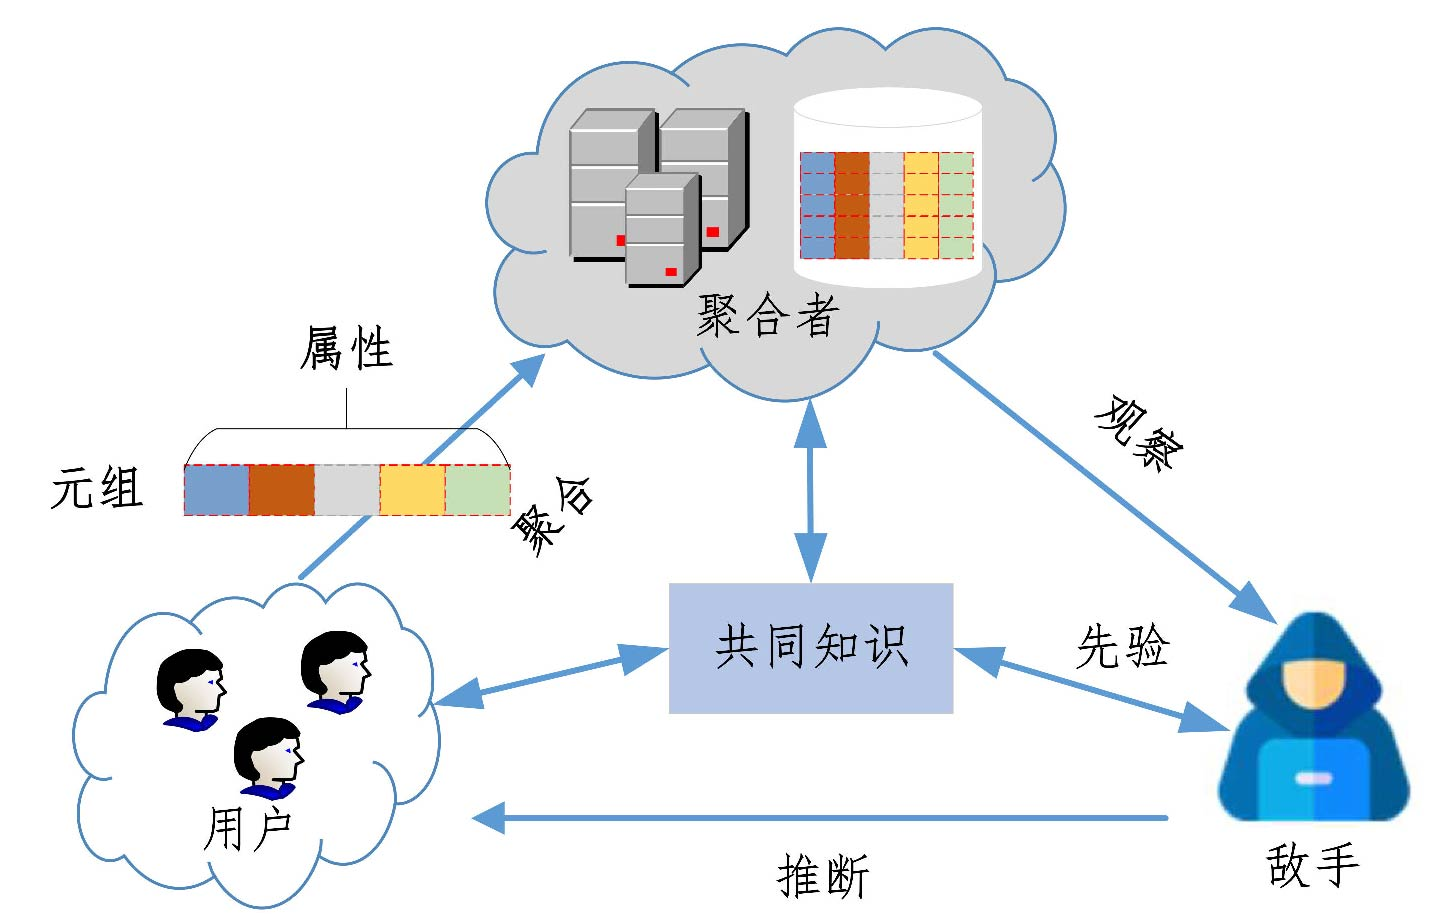
\includegraphics[width = 0.65\linewidth]{./figures/chapter06/chapter06_1.jpg}
	\caption{面向多维数据收集的系统模型}
	\label{fig:chapter06_Fig01}
\end{figure}

不失一般性,本章中所考虑的攻击模型是一个半诚实(Semi-honest)的敌手模型,也即是,聚合者诚实的执行隐私协议,但是偏好于从每一个报告的伪装数据中推断用户的私密信息。基于此,本章中假设聚合者可以观察这些报告数据,并已经事先知道了数据字母表和先验分布,这个假设捕捉到了一个消息灵通的敌手能力。本章中,数据字母表上的先验概率分布被假设为敌手和用户知道的共同知识。在这样的情况下,本章研究面向多维数据处理的最优隐私保护机制问题。

\subsection{问题提出}\label{sec:chapter06_problem_statement}
基于上图\ref{fig:chapter06_Fig01}中所示的系统模型,假设系统中有~$n$~个用户,$[n]=\{1,2,\cdots,n\}$,并且~$n$~可以是一个足够大的整数。随机变量~$X^i$表示第~$i$~$(1\leq i \leq n)$个用户的私密数据,随机向量$\bm{X}$表示用户的私密数据。更多的,假设每一个用户的数据包含有$d$个属性,记作$\bm{A}=\{A_1,A_2,\cdots,A_d\}$。此外,令$\mathcal{X}_j$是一个有限离散集合,表示第~$j$~$(1 \leq j \leq d)$个属性的所有可能的取值,也即是,属性$A_j$的域。相似的,$\hat{\mathcal{X}}_j$是一个有限离散集合,表示属性$A_j$的扰动数据取值域。进一步,使用$\mathcal{X}_j=\{1,2,\cdots,|\mathcal{X}_j|\}$表示属性$A_j$域中的离散字母符号,其中$|\mathcal{X}_j|$是$\mathcal{X}_j$的基数。由此,笛卡尔积$\mathcal{X}_1\times \mathcal{X}_2\times \cdots \mathcal{X}_d$有$\prod_{j=1}^{d}|\mathcal{X}_j|$个可能的取值,记作$\mathcal{X}=\prod_{j=1}^{d}\mathcal{X}_j$表示一个有限域,称为数据全集。除此之外,本章中使用~$x$~和~$\bm{v}~$分别表示个体数据的单个属性和元组。基于上述的符号表示,以下正式的表述本章中的研究问题。


给定一个用户有关的元组数据,本章的研究问题是寻找一个最优隐私保护机制集合,用于生成一个报告的伪装元组。这个问题被正式的定义为问题\ref{pro:chapter06}。

\begin{problem}\label{pro:chapter06}
对于给定的$n$个用户和每个用户的$d$维私密数据$\bm{v}=(v_1,v_2,\cdots,v_d)$。为了保护隐私,真实的元组应该被扰动获得一个混淆的元组$\bm{v}'=(v_1',v_2',\cdots,v_d')$同时保持数据的可用性。由此,这个问题是寻找一个最优的隐私保护机制集合$\{Q_j\}_{j=1}^d(Q_j \in \mathcal{Q}_{d,\tau})$,对于不同属性敏感等级,在质量损失约束的条件下,最小化隐私泄露。
\end{problem}

为了解决上述提出的问题\ref{pro:chapter06},本章中利用信息论的方法提出了ORRP的解决方案。接下来,给出方案具体的细节描述。

\section{隐私保护数据收集方案}\label{sec:chapter06_our_scheme}

本节中阐述提出的多维数据收集ORRP方案。首先,\ref{subsec:our_idea}小节概述本章的研究方案。然后,\ref{subsec:MI_optimal_mechanism}和\ref{subsec:ORRP}小节给出详细的方案描述。

 \subsection{研究方案概述}\label{subsec:our_idea}

不失一般性,用户的数据被考虑为包含数值型和类别型属性的混合数据类型。由此,这种特殊的数据结构和不同的隐私敏感度需求将会给隐私保护机制带来以下三个主要的挑战。

\begin{itemize}
\item 为了处理用户的隐私偏好,不同的属性应该被考虑具有不同的敏感度需求。由于这样的隐私需求,属性级的隐私保护需要有区分的保护强度,这成为了隐私保护机制设计的一个挑战。

\item 隐私保护机制应该解决一个关键的问题,那就是隐私保护和质量损失的权衡问题(信噪比的问题\cite{zhang2014privbayes})。解决上述问题需要寻找一个最优的隐私机制满足本章中原始的目标。而且,在寻找最优隐私机制的过程中计算复杂性应该是可以接受的。

\item 多维数据可能是更高维度的数据(如$30$个属性或者更多),有效的数据可能是稀疏的。多维和数据稀疏的问题将会降低隐私保护机制的性能,也即是,减少数据的可用性和数据处理的效率。
\end{itemize}

在设计面向多维数据的隐私保护机制时,应该解决上述的挑战。为了解决上述的挑战进而获得本章的目标,使用信息论的方法提出ORRP方案。对于提出的方案介绍主要包含有两部分:分别是隐私保护的数据收集方案和隐私与效用的分析。接下来,首先展现所提出方案的一个概览,然后提供更多的具体实现细节。

(1) 隐私保护数据收集方案。本章中提出的ORRP方案主要有两个阶段组成,如图\ref{fig:chapter06_Fig02}中描述。两个阶段分别是寻找互信息隐私最优机制和多维数据的有序随机响应扰动。在第一阶段中,元组属性拆分,形式化属性的最优化模型寻找最优的概率密度函数,进一步,提出算法\ref{alg:B-A}求解最优化模型。更多的细节,在\ref{subsec:MI_optimal_mechanism}小节进行介绍。第二个阶段中,将一维数据的处理推广到多维数据情景,提出了ORRP方案,进一步,设计对应的实现算法\ref{alg:ORRP}。方案的设计和实现细节在\ref{subsec:ORRP}小节进行介绍。与此同时,分析了提出的方案以及实现算法的计算复杂性。

(2) 隐私与数据质量分析。从隐私泄露、质量损失和相关度损失方面对提出的方案性能进行分析。首先,基于不可区分等级和互信息隐私泄露分析了所提出方案的隐私泄露,理论分析的结果在\ref{subsec:privacy_analysis}节给出具体的介绍。其次,扰动数据的质量评估在\ref{subsec:utility_evalution}节进行分析。最后,在\ref{subsec:correlated_degree_loss}节叙述了相关度的损失分析。


\begin{figure}[htbp]
	\centering
	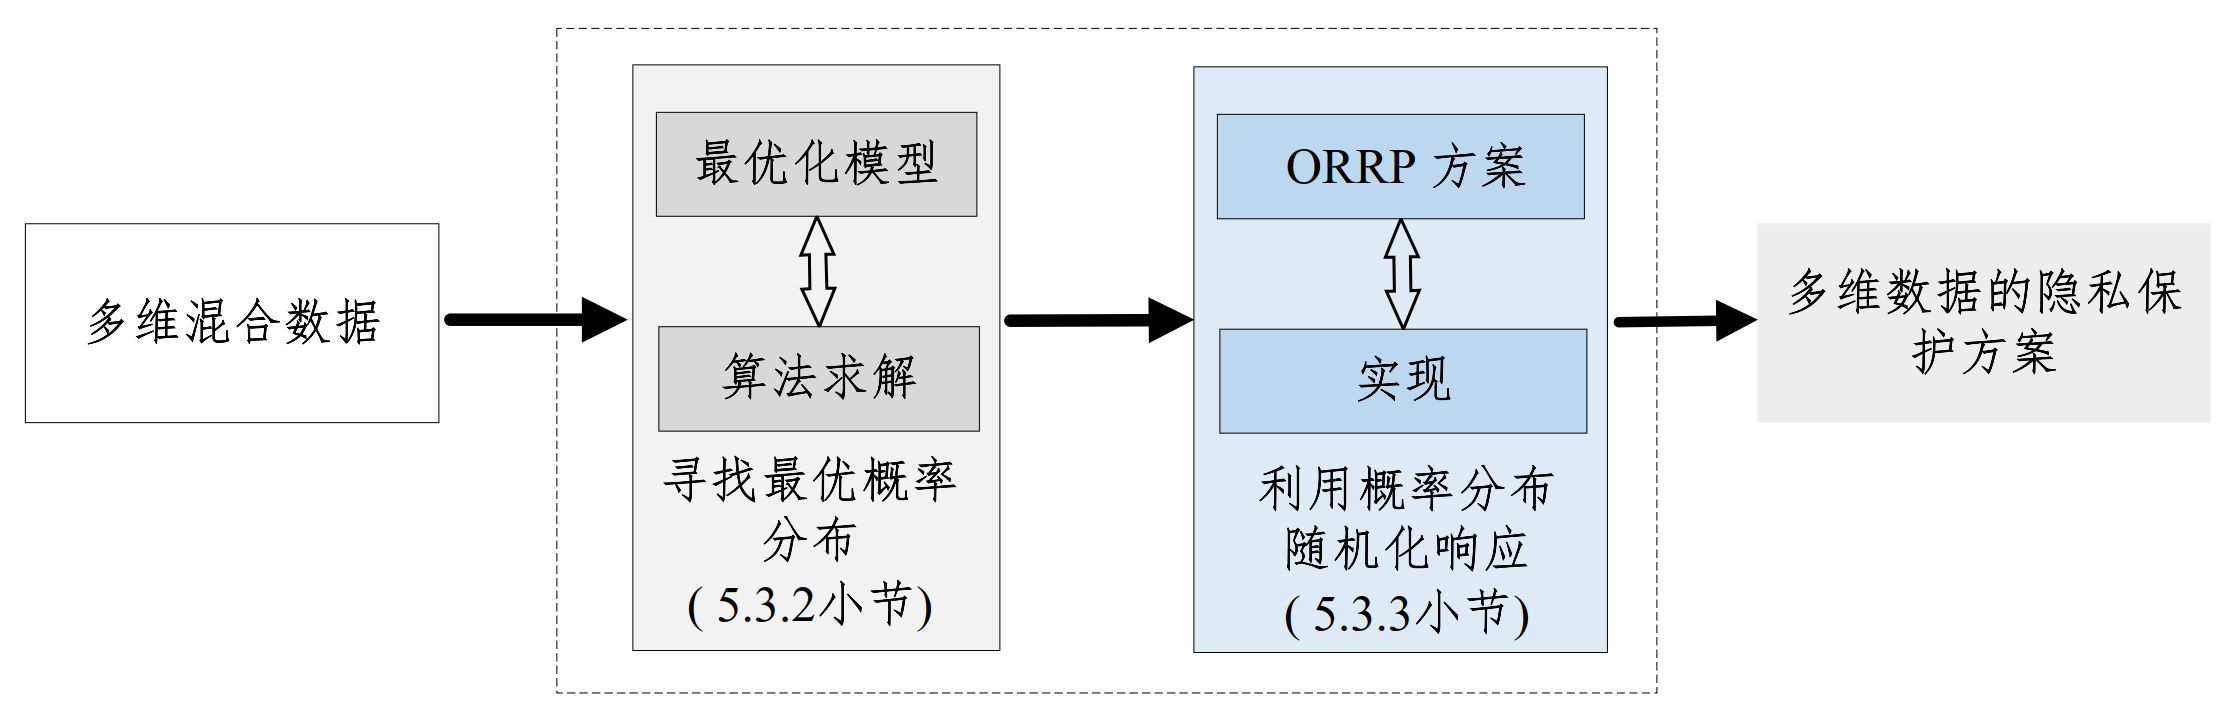
\includegraphics[width = 0.99\linewidth]{./figures/chapter06/chapter06_2.jpg}
	\caption{ORRP方案实现的两个阶段}
	\label{fig:chapter06_Fig02}
\end{figure}

\subsection{互信息隐私最优机制}\label{subsec:MI_optimal_mechanism}

为了更好的描述针对多维数据提出的有序随机响应扰动(ORRP)方案,本小节中首先给出利用优化模型计算单属性最优隐私机制的方法。随后,在\ref{subsec:ORRP}小节中阐述将本节的理论结果推广应用到多维数据的情况。


离散随机变量$X_j$和$\hat{X}_j$分别表示属性$A_j$的真实私密敏感数据和隐私保护后的伪装数据。隐私机制的概率性映射$\mathcal{X}_j \xrightarrow{Q_j} \hat{\mathcal{X}}_j$,可以被视为一个噪声信道$Q_j$,也即是一个损失压缩机制。对于$X_j$属性的每一个用户私密数据$x$,隐私保护机制$Q_j$生成伪装数据$\hat{x}$使用条件概率密度函数$q(\hat{x}|x)$。基于此,本章中使用$p(x)$表示$\hat{\mathcal{X}}_j$上的先验分布,并假设所有的用户数据独立同分布的抽样于一个潜在的分布。而且,假设分布$p(x)$是用户和敌手已知的共同知识。基于这样的假设,本章中考虑隐私泄露和数据质量的信息论度量。首先,使用$X_j$与$\hat{X}_j$之间的互信息$I(X_j;\hat{X}_j)$测量敌手的信息增益,也就是在观察到扰动数据$\hat{x}$后有关原始数据$x$的不确定度减少量。依据文献\mycite{oya2017back},互信息度量隐私泄露有一个具体明确的解释,它表示保证敌手能够完全的识别出个体私密数据$x$的平均意义上需要的比特数。基于此,最小化互信息隐私泄露可以有效阻止用户的私密数据被推断。其次,伪装数据用于表示原始数据的质量由一个失真函数测量,记作$d(x,\hat{x})$。然后,本章的目标就是计算隐私机制的条件概率密度函数,在满足数据质量损失约束$\tau$的条件下,使得互信息隐私泄露最小化。重要的是,可以通过缩放$\tau$表示不同属性的失真需求,这将在\ref{subsec:ORRP}小节中进一步讨论。在此,将寻找$Q_j \in \mathcal{Q}_{d,\tau}$的问题形式化表述为以下的凸优化模型求解问题。
\begin{alignat}{2}
  R(\tau)  & =\min_{q(\hat{x}|x)} I(X_j;\hat{X}_j) \label{min:lp1}  \nonumber\\
   \mbox{subject to} \quad
   & \sum_{x}\sum_{\hat{x}}p(x)q(\hat{x}|x)d(x,\hat{x})\leq\tau \\
   & \sum_{\hat{x}} q(\hat{x}|x)=1,\forall x\in \mathcal{X}_j \\
   & q(\hat{x}|x)\geq 0,\forall x \in \mathcal{X}_j,\hat{x}\in \hat{\mathcal{X}}_j
   \end{alignat}

上述优化模型的形式化表述和著名的率失真理论(更多细节,参考文献\mycite{cover2006elements})具有相同的形式\cite{wang2016on}。本质上来说,上述研究问题规约为一个信道有损压缩问题。针对上述优化模型,可以利用拉格朗日乘子法求解,并且该方法已经在很多的研究工作中得到了应用。在此,本节中省略掉了拉格朗日函数的具体计算过程,直接借用文献\mycite{cover2006elements}中的计算结果,其中的最优解的结果使用凸问题的Karush-Kuhn-Tucker(KKT)最优性条件\cite{boyd2004convex}。基于此,互信息隐私的最小化则有以下结论

 \begin{equation}\label{Eq:opt_prob}
 q(\hat{x}|x)=\frac{q(\hat{x})e^{-\lambda d(x,\hat{x})}}{\sum_{\hat{x}}q(\hat{x})e^{-\lambda d(x,\hat{x})}}
 \end{equation}
其中,$\lambda$是拉格朗日乘子,$q(\hat{x})$是$\hat{\mathcal{X}}_j$上的后验概率分布。

进一步,注意到上述公式~\ref{Eq:opt_prob}表述的最优条件概率密度函数$q(\hat{x}|x)$有一个指数形式。通常情况下,直接通过拉格朗日乘子法计算最优的概率密度函数是困难的。为了解决这个问题,Blahut\cite{blahut1972computation}和Arimoto\cite{arimoto1972an}提出Blahut-Arimoto(B-A)算法计算最优的概率密度函数。B-A算法的基本思想是在两个概率分布集合之间交替最小化,其中使用Kullback-Leibler散度测量两个分布之间的距离。更重要的,Csisz\'{a}r\cite{csiszar1974on,csiszar1984information}已经证明了率失真函数的极限,存在于交替最小化的过程中。近些年,B-A算法已经被应用于基于位置的隐私保护机制设计中\cite{oya2017back,zhang2019online}。作为本章内容的一个基本理论支撑,利用一些合适选择的参数$\lambda$,率失真函数的曲线可以被描绘出来。特别的,率失真函数$R(\tau)$在期望的失真和拉格朗日乘子上有一个重要的性质。

\begin{theorem}\label{theorem:chapter06_01}
	率失真函数$R(\tau)$是一个有关失真门限$\tau$的凸的,且非增的函数,其曲线斜率是拉格朗日乘子$\lambda$。
\end{theorem}

由于篇幅的限制,本章中省略定理\ref{theorem:chapter06_01}的具体证明过程,如需要可参考文献\mycite{cover2006elements}中引理10.4.1的证明过程。

基于上述的定理\ref{theorem:chapter06_01},设置不同的$\lambda$可以获得率失真$R(\tau)$的曲线。接下来,通过以B-A算法为基础结合本章的应用,解决上述的优化模型。具体地实现细节如算法\ref{alg:B-A}中的伪代码描述,其主要包含有以下三个关键的计算步骤。

\begin{itemize}
	\item [(1)] 首先,算法序列化属性$A_j$的取值域$\mathcal{X}_j$为离散化序列$1,2,\cdots,|\mathcal{X}_j|$,即是,将属性域值映射到一个整型的序列数。然后,算法根据输出域的基数值初始化$r_0(\hat{x})$为均匀分布(算法\ref{alg:B-A}的$1 \sim 2$ 行)。
	
	\item [(2)] 其次,依据公式\ref{Eq:opt_prob},算法使用$r_0(\hat{x})$计算条件概率$q_0(\hat{x}|x)$。在获得$q_0(\hat{x}|x)$之后,计算一个初始的互信息$I_0$,并重新计算$r(\hat{x})=\sum_{x}p(x)q_0(\hat{x}|x)$(算法\ref{alg:B-A}的$3 \sim 5$行)。
	
	\item [(3)] 最后,算法重复的更新$q(\hat{x}|x)$和$r(\hat{x})$直到收敛(算法\ref{alg:B-A}的$6\sim 15$行)。
\end{itemize}
\begin{algorithm}[htb]
 \small
 \setstretch{1.3}
\caption{基于B-A的最优化隐私机制}
\label{alg:B-A}
\begin{algorithmic}[1]
\REQUIRE
\begin{tabular}[t]{p{3mm}l}
 $A_{j}$&: $d$-维属性的第$j$个属性$(1 \leq j \leq d)$\\
 $\mathcal{X}_j$&: $A_j$的属性域 $(1 \leq j \leq d)$\\
 $\lambda$&: 拉格朗日乘子\\
 $T$&: 算法收敛门限参数
\end{tabular}
\ENSURE$|\mathcal{X}_j|$-维条件概率$Q_j$

\STATE 初始化域$\mathcal{X}_j$到一个序列$1,2,\cdots,|\mathcal{X}_j|$
\STATE 初始化先验概率分布$p(x)$,$|\mathcal{X}_j|$-维失真$d(\hat{x},x)$,均匀分布$r_0(\hat{x})$
\STATE 计算$q_0(\hat{x}|x)=\frac{r_0(\hat{x})e^{-\lambda d(\hat{x},x)}}{\sum_{\hat{x}}r_0(\hat{x})e^{-\lambda d(\hat{x},x)}}$
\STATE 计算互信息$I_0=\sum_{x,\hat{x}}p(x) q_0(\hat{x}|x)\log\frac{q_0(\hat{x}|x)}{r_0(\hat{x})}$
\STATE 计算 $r(\hat{x})=\sum_{x}p(x)q_0(\hat{x}|x)$.
\WHILE{true}
\STATE 计算$q(\hat{x}|x)=\frac{r(\hat{x})e^{-\lambda d(\hat{x},x)}}{\sum_{\hat{x}}r(\hat{x})e^{-\lambda d(\hat{x},x)}}$
\STATE 计算互信息$I=\sum_{x,\hat{x}}p(x) q(\hat{x}|x)\log\frac{q(\hat{x}|x)}{r(\hat{x})}$
\IF{$I_0-I\leq T$}
%最小互信息量,期望失真,设计矩阵都有了
\STATE 设置$Q_j = q(\hat{x}|x)$
\ELSE
\STATE 设置$I_0=I$
\STATE 计算$r(\hat{x})=\sum_{x}p(x)q(\hat{x}|x)$
\ENDIF
\ENDWHILE
\RETURN $Q_j$
\end{algorithmic}
\end{algorithm}

上述算法针对本章中的单属性最优化模型进行求解,算法执行完成则可以获得单个属性的最优条件概率分布$q(\hat{x}|x)$,也即是,最优的互信息隐私机制$Q_j$。在此,针对上述算法产生的隐私机制给出几点备注说明。

\begin{remark}{\em
	通过上述算法获得的隐私机制提供一个确定等级的隐私保证\textup{\cite{oya2017back,wang2016on,mir2012information}}。它同时也满足一个扩展的差分隐私概念,提供$\epsilon$-geo-indistinguishability。本章中省略去具体的证明过程,其证明过程类似于文献\textup{\mycite{oya2017back}}附录中的证明。}
\end{remark}

\begin{remark}{\em
隐私机制(如LDP,$d_{\mathcal{X}}$-privacy)的定义独立于用户的数据和先验分布。由此,一个自然的问题表述为
\begin{question}
上述算法\textup{\ref{alg:B-A}}在计算最优化隐私机制时,是否已经泄露了用户的隐私?
\end{question}
首先,这个问题是可以解决的,但是解决的方法与文献}\mycite{wang2020publishing}{\em 中注入少量的噪声有所区别。本章中,信息论的方法同时考虑论隐私机制$Q_j$ 和先验分布$p(x)$。其次,上述算法}\ref{alg:B-A}{\em 解决提出的优化问题仅需要$p(x)$而不是真实的用户数据。换句话说,算法仅需要用户和敌手已知的共同知识进行计算。实践中,这个计算的任务可以在云上或委托给第三方代理完成。}

\end{remark}

\begin{remark}{\em 接下来,给出上述算法的计算复杂性分析。首先,算法}\ref{alg:B-A}{\em 的计算复杂性主要花费在迭代的重复计算。对于每一轮的迭代,算法需要$|\hat{\mathcal{X}}_j|$次计算对于一个特定的符号$x$计算$q(\hat{x}|x)$,由此,计算需要$O(|\hat{\mathcal{X}}_j|)$次基本操作。进一步,考虑所有$\mathcal{X}_j$中的符号,计算$q(\hat{x}|x)$的计算复杂度将会是$O(|\mathcal{X}_j||\hat{\mathcal{X}}_j|)$,也即是$O(|\mathcal{X}_j|^2)$。另外,互信息和$r(\hat{x})$的计算复杂性需要$O(|\hat{\mathcal{X}}_j|)$对于每一个符号$x \in \mathcal{X}_j$,由此,计算$r(\hat{x})$的计算复杂性总共是$O(|\mathcal{X}_j|^2)$。}
\end{remark}


\subsection{有序随机响应扰动机制}\label{subsec:ORRP}

上述讨论了单个属性$X_j$的最优隐私机制求解问题。接下来,将上述处理思想推广应用到包含数值型和类别型属性的多维数据情景。首先,使用$X^i$表示一个元组拥有$d$个属性的第$i$个用户数据。然后,本节的目标是基于\ref{subsec:MI_optimal_mechanism}小节提出有序随机响应扰动(ORRP)方案,并使用ORRP获得一个扰动的元组$\hat{X}^i$。以下介绍方案实现的细节。

在ORRP方案设计的阶段,有一些问题需要考虑。首先,多维的数据或许有很多的属性(例如$30$个或更多),多维的属性将会给隐私机制带来挑战。这样的情况下,降维的方法是处理多维数据时通常采用的方法\cite{ren2018textsf,zhang2014privbayes}。其次,属性之间可能存在着关联,这种存在的关联和相关度是可以通过皮尔逊相关系数\cite{zhu2015correlated}和互信息\cite{chen2015differentially}进行测量的。最后,这些属性可能存在着不同的隐私敏感度需求。为了处理用户的隐私偏好,这些多维属性应该被考虑具有不同的隐私敏感程度\cite{murakami2019utility,gu2020providing}。基于上述的分析和受到文献\mycite{wang2019collecting,andres2013geo}的启发,本章中提出ORRP方案实现整个数据元组的随机扰动。

本章提出ORRP方案的基本思想是将每一个数据元组划分为多元随机变量,其过程如图\ref{fig:chapter06_Fig03}描绘。然后,ORRP使用上文中算法\ref{alg:B-A}计算输出的最优隐私机制的概率密度函数有序随机扰动每一个属性值。对于真实的数据元组$\bm{v}=(v_1,v_2,\cdots,v_d)$中的每一个属性值$v_j$独立的应用隐私机制$Q_j$获得扰动的伪装值$v'_j$。进一步,连接每一个扰动的属性值获得一个扰动的元组,也就是,连接每一个$v'_j$得到扰动的元组$\bm{v}'=(v'_1,v'_2,\cdots,v'_d)$。为了清晰地说明上述处理思想,首先给出一个具体实例。

\begin{figure}[htbp]
	\centering
	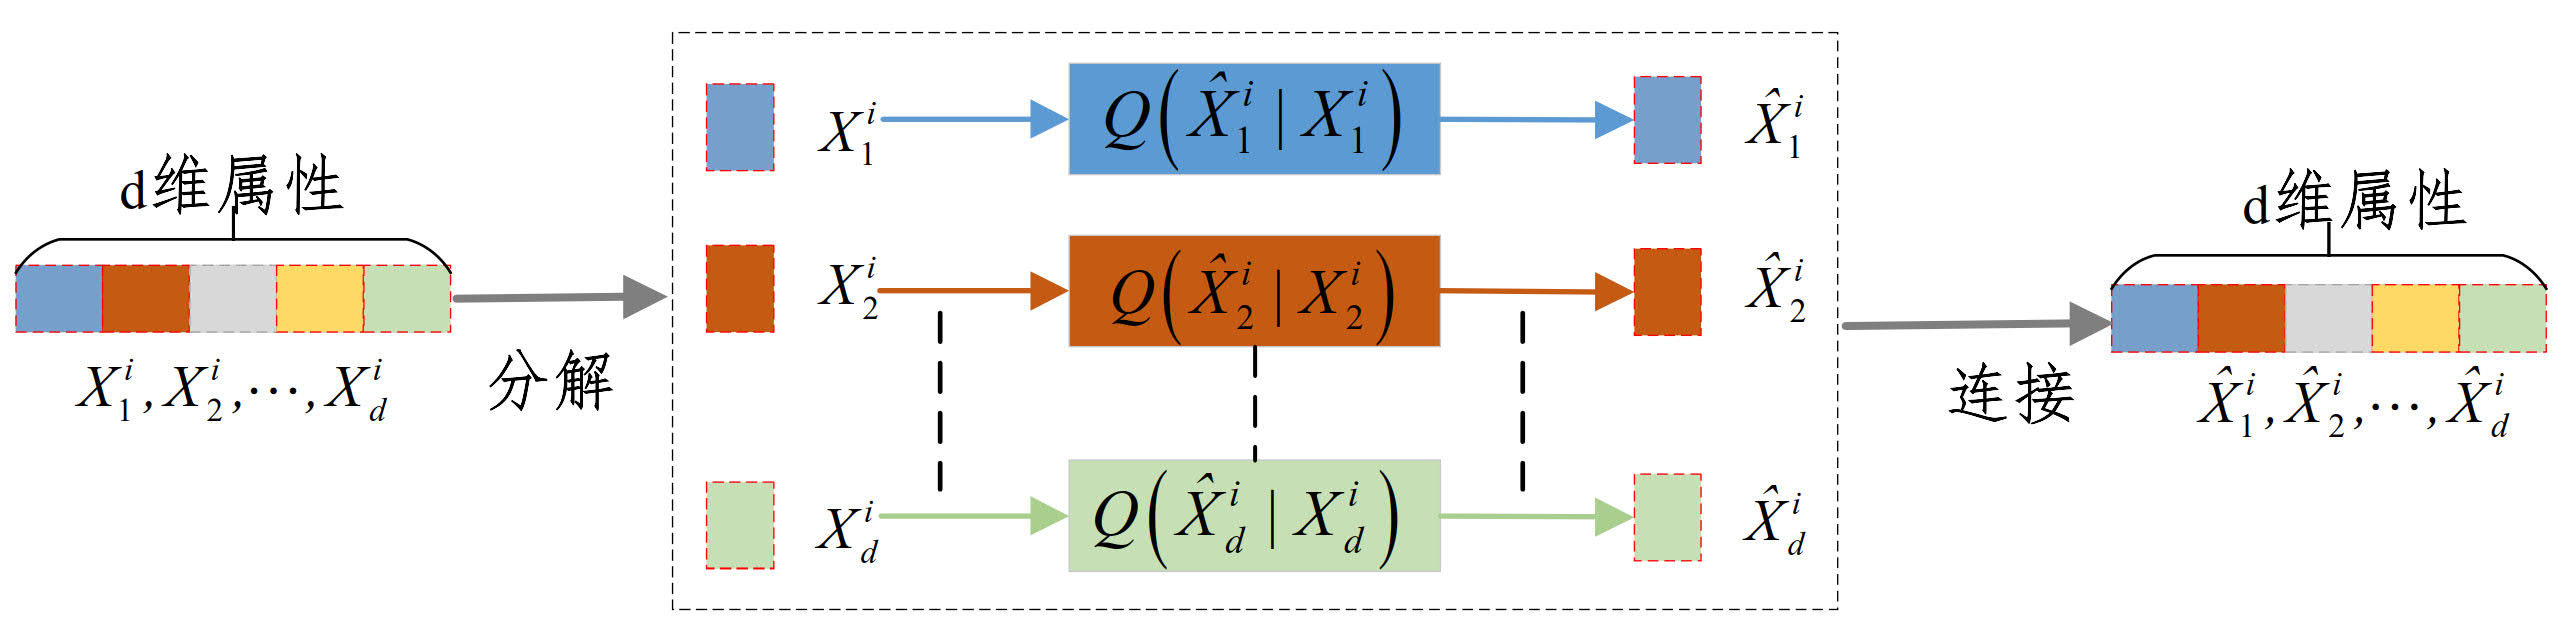
\includegraphics[width = 0.8\linewidth]{./figures/chapter06/chapter06_3.jpg}
	\caption{ORRP方案对多维数据的有序随机扰动}
	\label{fig:chapter06_Fig03}
\end{figure}

\begin{example}
	对于\textbf{Adult}\footnote{http://archive.ics.uci.edu/ml/datasets.php\label{ft:UCI}}数据集并从属性集合中选择\{``Age'',``Education'',``Marital-status''	,``Gender''\}$4$个属性。如果一个特定的个体数据元组是\{39, Bachelors, Never-married, Male\},将其拆分为多个属性值,并借用键值型的概念将它们表示为 \{``Age'': 39\}, \{``Education'': Bachelors\}, \{``Marital-status'': Never-married\} 和 \{``Gender'': Male\}。然后,考虑每一个属性的随机响应映射到自身的值域。否则,扰动的结果将丢失原始的语义。为此,随机的生成扰动的属性值使用每一个属性的最优概率分布。例如,可能获得一组扰动值 \{``Age'': 30\}, \{``Education'': Masters\},\{``Marital-status'': Never-married\} 和 \{``Gender'': Female\},最后连接这些扰动的结果,得到伪装的元组数据 \{ 30, Masters, Never-married, Female\}。
\end{example}

接下来,考虑属性级隐私敏感性的概念。如本章引言中示例介绍的婚姻状态和疾病信息,具有不同的隐私偏好,本章中假设所有的用户达成一致协议具有共同的认知。在个性化的隐私需求\cite{murakami2019utility}方面也依然是未来的研究方向,留给进一步的研究工作。本章中,多属性之间可以有一个偏序关系($\succcurlyeq$)去表达用户隐私偏好强度。首先,回顾上文\ref{subsec:MI_optimal_mechanism}中单个属性的最优化问题,其中数据质量由损失约束$\tau$控制。直观地说,越高的期望失真$\mathbb{E}[d(X_j;\hat{X}_j)]$具有越好的混淆程度,这可以解释为失真程度较高表示报告的伪装数据$\hat{X}_j$与原始的数据$X$之间的不相关度越大,也就是数据质量几乎为零。综合上述因素考虑,对于不同的属性级敏感度可以通过适当的缩放约束条件$\tau$可以获得一个由单属性最优机制$Q_j$组成的隐私机制集合$\{Q_j\}_{j=1}^{d}$。然后,利用集合中的隐私机制$Q_j$依此实现对属性有区分性的保护。以下考虑对所有的用户执行相同的处理流程,在获得元组扰动的隐私机制$\{Q_j\}_{j=1}^{d}$之后,实现ORRP方案的关键是计算一个扰动的数据元组。图4展示了提出的ORRP方案数据元组扰动流程,包含有两个主要阶段,第一个阶段是元组属性分解并利用单属性最优化模型计算概率分布函数问题,由算法\ref{alg:B-A}实现。第二个阶段,利用前一阶段的分布函数有序扰动用户数据,获得扰动数据元组,由以下算法\ref{alg:ORRP}实现。

\begin{figure}[htbp]
	\centering
	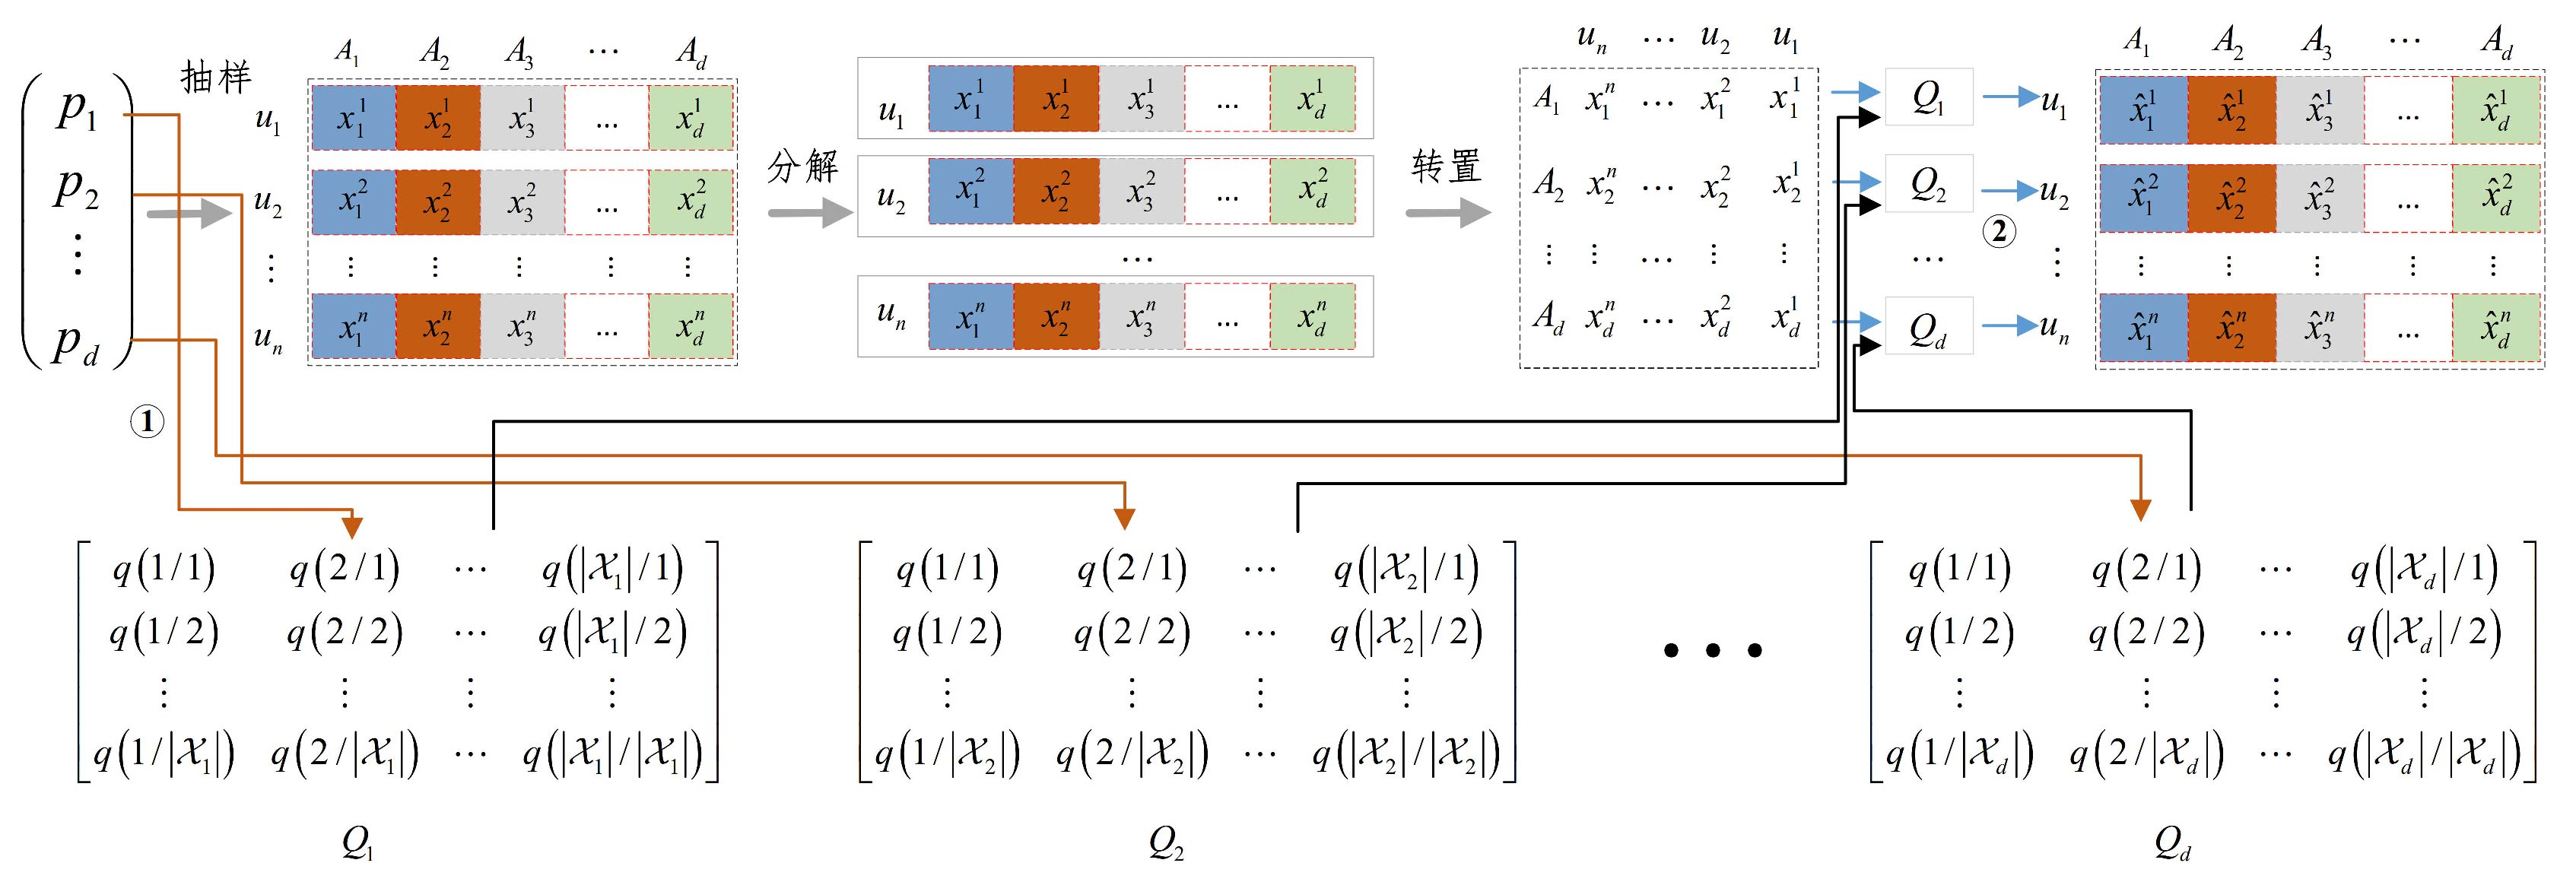
\includegraphics[width = 0.99\linewidth]{./figures/chapter06/chapter06_4.jpg}
	\caption{多维数据有序随机扰动的两个阶段示意图}
	\label{fig:chapter06_Fig04}
\end{figure}

%算法

图~\ref{fig:chapter06_Fig04}中描绘了所提ORRP方案的原理和流程,接下来,针对提出的ORRP介绍相应的算法实现,如算法\ref{alg:ORRP}伪代码描述。随后,给出算法的计算效率和特性的分析。

\begin{algorithm}[htbp]
 \small
 \setstretch{1.3}
\caption{ORRP方案算法伪代码}
\label{alg:ORRP}
\begin{algorithmic}[1]
\REQUIRE
\begin{tabular}[t]{p{3mm}l}
 $\bm{A}$&: 属性集合, i.e., $\bm{A}=\{A_1,A_2,\cdots,A_j,\cdots,A_d\}$\\
 %$Q_j$&: the optimal privacy mechanism for $j$-th attribute,\\
 $\bm{v}$&: $d$-维的元组 \\
 & i.e., $\bm{v}=(v_1,v_2,\cdots,v_j,\cdots,v_d)$, $(1\leq j\leq d)$
\end{tabular}
\ENSURE $\bm{v}'=(v_1',v_2',\cdots,v_j',\cdots,v_d')$: 报告扰动元组$\bm{v}$
\STATE 利用算法\ref{alg:B-A}计算最优隐私机制集合$\{Q_j\}_{j=1}^d$
\STATE 拆分一个元组$\bm{v}$为$d$-维属性值, i.e., $v_1,v_2,\cdots,v_d$ \\ /*有序随机响应每一个属性值$A_j$*/
\FOR{each $j=1,2,\cdots,d$}
\STATE 依据算法\ref{alg:B-A}的第$1$行,计算$v_j$在域$\mathcal{X}_j$中的一个序列号$k$
\STATE 根据概率分布$Q_{j}$的第$k$行,随机响应一个序列号$\hat{k}$,记作$Q_{j}^{k}$ \\
/*随机响应一个扰动的值保持相同的域*/
\STATE 重构域$\mathcal{X}_j$中第$\hat{k}$个元素获得扰动结果$v_j'$
\ENDFOR
\STATE 连接属性$A_j\in \bm{A}$的每一个扰动结果获得扰动的元组结果$v_1',\cdots,v_d'$
\RETURN $\bm{v}'=(v_1',v_2',\cdots,v_j',\cdots,v_d')$
\end{algorithmic}
\end{algorithm}

上述算法\ref{alg:ORRP}的伪代码描述中,主要包含有以下的三个步骤:

\begin{itemize}
	\item[(1)] 首先,针对单属性$X_j$利用子算法\ref{alg:B-A}获得单属性的最优隐私机制$\{Q_j\}_{j=1}^{d}$,即是通过优化模型求解的条件概率密度函数(算法\ref{alg:ORRP}的第$1$行)。
	
	\item [(2)] 其次,算法拆分一个元组$\bm{v}$为$d$-维属性值,并计算属性值映射到取值域$\mathcal{X}_j$的序号。然后,使用$Q_j$随机的扰动报告一个序号$\hat{k}$。在获得报告序号$\hat{k}$之后,算法将其映射到输出域中的一个扰动值$v_{j}'$。进一步,对所有的属性重复执行这些过程,得到各属性扰动的伪装值(算法\ref{alg:ORRP}的第$2\sim 7$行)。
	
	\item[(3)]最后,算法连接所有的报告数据$v_j'$,返回扰动的伪装元组数据$\bm{v}' = (v_1',v_2',\cdots,v_d')$ (算法\ref{alg:ORRP}的第$8$和$9$ 行)。
\end{itemize}

\begin{remark}{\em
	通过一些基本的操作分析算法}\ref{alg:ORRP}{\em 的计算复杂性。首先,对于每一个属性$A_j(1\leq j \leq d)$,前文中}\ref{subsec:MI_optimal_mechanism}{\em 小节介绍的算法}\ref{alg:B-A},{\em 其计算复杂度是$O(|\mathcal{X}_j|^2)$。为了获得最优的隐私机制集合$\{Q_j\}_{j=1}^{d}$,算法的计算复杂度将是$O(\sum_{j=1}^{d}|\mathcal{X}_j|^2)$。之后,算法在序号与域值之间建立一个一对一的映射,用于生成扰动数据。算法执行这个过程开销是$O(d)$。因此,算法}\ref{alg:ORRP}{\em 的计算复杂度是$O(d)+O(\sum_{j=1}^{d}|\mathcal{X}_j|^2)$。}
\end{remark}

本章中提出的ORRP方法和Wang等\cite{wang2019collecting}提出的分段机制(PM)对于多维数据的处理方式有所不同。首先,Wang等的PM方法通过将所有的属性看作为等价敏感的,分配隐私参数$\epsilon/d$,然后,所提出的隐私机制在多维属性总体上提供$\epsilon$隐私保护。然而,本章中提出的ORRP扰动方法提供的隐私保护不可区分等级与拉格朗日乘子参数密切相关,总体隐私水平由差分隐私的序列组合定理\cite{dwork2014algorithmic,mcsherry2007mechanism}保证。


\begin{theorem}\label{theorem:chapter06_sequence}
给定一组隐私机制$\{Q_j\}_{j=1}^{d}$,其中的每一个隐私机制$Q_j:\mathcal{X}\rightarrow\hat{\mathcal{X}}_j$提供$\epsilon_j d_{\mathcal{X}}$-privacy保护,则有隐私机制$\{Q_j\}_{j=1}^{d}$提供$\sum _{j=1}^{d} \epsilon_j d_{\mathcal{X}}$-privacy。
\end{theorem}

另外,理论方面对比两个先进的隐私机制,所提出的ORRP方案具有两个特点。首先,相较于文献\mycite{wang2019collecting}中的方法,本章中的ORRP方案不需要区分数值型和类别型属性,并可以在第一个阶段时通过缩放参数计算不同属性的扰动条件概率函数,为属性提供不同等级的隐私保护。其次,提出的方案对每一个属性$X_j$使用相对应的隐私机制$Q_j$获得报告的元组,和文献\mycite{andres2013geo}中为元组的每一个值应用相同的隐私机制有所不同。

\section{隐私与效用分析}\label{sec:chapter06_privacy_utility_analysis}

本节中通过分析隐私泄露、数据质量和相关度损失评估提出的隐私机制。具体来说,\ref{subsec:privacy_analysis}小节分析隐私泄露,\ref{subsec:utility_evalution}小节给出数据质量的分析、\ref{subsec:correlated_degree_loss}小节量化隐私机制对多维属性之间相关性损失的影响。

\subsection{隐私分析}\label{subsec:privacy_analysis}
首先,$\epsilon$不可区分等级是量化、分析隐私机制隐私保护强度的事实标准。对于所提出的有序随机扰动方案,每一个属性的最优隐私机制$Q_j$是单属性优化模型的解,并由算法\ref{alg:B-A}计算条件概率分布得到。特别的,文献\mycite{oya2017back}指出这种方式获得的隐私机制提供泛化推广的$\epsilon_j$-geo-indistinguishability保护。由此,对于属性$A_j$由隐私机制$Q_j$提供的隐私等级是$\epsilon_j$,所以,基于上述组合定理\ref{theorem:chapter06_sequence},本章中提出的ORRP机制提供$\sum_{j=1}^{d}\epsilon_j$-geo-indistinguishability。其次,使用互信息(MI)量化平均意义上的信息泄露,对于每一个属性$A_j$的随机变量$X_j$,独立的使用隐私机制$Q_j$扰动得到伪装数据,$\hat{X}_j$表示。由此则有

\begin{equation}
	I(X_j;\hat{X}_j)=\sum_{x\in\mathcal{X}_j}\sum_{\hat{x}\in\hat{\mathcal{X}}_j}p_j(x)q_j(\hat{x}|x)\log\frac{q_j(\hat{x}|x)}{q_j(\hat{x})}
\end{equation}
其中 $p_j(x)$ 和 $q_j(\hat{x}|x)$ 分别表示先验分布和条件概率分布。

\begin{theorem}\label{theorem:upper bound} 对于多维属性变量$\bm{X}=\{X_1,X_2,\cdots,X_d\}$,有序使用隐私机制$\mathcal{Q}=\{Q_j\}_{j=1}^{d}$ 扰动输出$\hat{\bm{X}}=\{\hat{X}_1,\hat{X}_2,\cdots, \hat{X}_d\}$,互信息隐私泄露量$I(\bm{X};\hat{\bm{X}})\leq \sum_{j=1}^{d}I(X_j;\hat{X}_j)$。
\end{theorem}

{\em 证明:首先,将用户数据元组分解为单属性分量,然后,ORRP隐私机制$\{Q_j\}_{j=1}^d$独立的应用每一个$Q_j$ 到每一个属性$A_j$,并顺序的随机响应每一个元组获得扰动混淆的元组。$\{Q_j\}_{j=1}^d$是各属性随机变量取值于不同字母表的独立并联信道模型。由此则有,提出的隐私机制条件概率乘积特性
	
	\begin{equation}
		q(\bm{\hat{x}|x})=\prod_{i=1}^{d}q(\hat{x}_j|x_j)
	\end{equation}
	其中的$q(\hat{x}_j|x_j)$表示第$j$个属性的隐私机制。 以此,根据条件熵的定义\textup{\ref{def:condition_entropy}},则有以下等式
	\begin{equation}
		H(\bm{\hat{X}|X})=\sum_{j=1}^{d}H(\hat{X}_j|X_j)
	\end{equation}
进一步,使用著名的互信息的性质,则有以下的公式
	
	\begin{equation}\label{eq:chapter05-1-14}
		I(\bm{X;\hat{X}})-\sum_{j=1}^{d}I(X_j;\hat{X}_j)=H(\hat{X}_1\hat{X}_2\cdots\hat{X}_d)-\sum_{j=1}^{d}H(\hat{X}_j)
	\end{equation}
然后,使用信息熵的性质可以容易的证明下面的不等式,也就是
	
	\begin{equation} \label{Inequality:MI}
		H(\hat{X}_1\hat{X}_2\cdots\hat{X}_d)\leq \sum_{j=1}^{d}H(\hat{X}_j)
	\end{equation}
基于上面的等式\textup{\ref{eq:chapter05-1-14}}和不等式\textup{\ref{Inequality:MI}},则有以下的不等式结论
	
	\begin{equation}
		I(\bm{X;\hat{X}})-\sum_{j=1}^{d}I(X_j;\hat{X}_j)\leq 0
	\end{equation}

	综合上述,可以得到互信息隐私泄露的上界是$\sum_{j=1}^{d}I(X_j;\hat{X}_j)$,当且仅当随机变量之间彼此相互独立,上式的等号成立。
}

基于上述定理\ref{theorem:upper bound},本章中使用分治划分的思想对于包含$d$-维属性的元组采用有序随机响应,在互信息隐私泄露方面满足下述的不等式结果
\begin{equation}\label{Eq:MI leakage}
	I(\bm{X};\bm{\hat{X}})\leq \sum_{j=1}^{d}I(X_j;\hat{X}_j)
\end{equation}
如此这样,不等式\ref{Eq:MI leakage}量化了隐私机制集合$\{Q_j\}_{j=1}^{d}$互信息隐私泄露的上界。

\subsection{效用分析}\label{subsec:utility_evalution}
隐私机制的效用分析是度量使用扰动后的伪装数据表示原始数据的质量。基于距离(如汉明距离\cite{kalantari2018robust,wang2016on}、欧几里德距离\cite{oya2017back})的度量是目前广泛使用的质量损失量化方法。本节中分析失真函数$d(x,\hat{x})$量化当真实数据为$x$报告扰动数据$\hat{x}$的数据质量。进一步,使用平均失真量化在平均意义上的数据质量损失。平均失真因具有直观且减少了算法的计算开销\cite{oya2017back}等优势,在一系列相关的研究工作中已经得到了应用得到了应用\cite{calmon2012privacy,andres2013geo,xiong2016randomized,oya2017back,wang2016on}。本节中,使用平均失真分析所提方案的数据质量。首先,对于单个属性有

\begin{equation}
	\mathbb{E}[d(X_j,\hat{X}_j)]=\sum_{x\in\mathcal{X}_j}\sum_{\hat{x}\in\hat{\mathcal{X}}_j}p_{j}(x)q_j(\hat{x}|x)d(x,\hat{x})
\end{equation}

\begin{theorem}\label{theorem:ED} 对于给定的单符号失真测量$d(x,\hat{x})$,多维随机变量$\bm{X}=\{X_1,X_2,\cdots,X_d\}$有序使用$\{Q_j\}_{j=1}^{d}$扰动得到$\hat{\bm{X}}=\{\hat{X}_1,\hat{X}_2,\cdots, \hat{X}_d\}$,其中$X_j \xrightarrow{Q_j} \hat{X}_j$,则有期望失真满足$\mathbb{E}[d(\bm{X},\hat{\bm{X}})]=\sum_{j=1}^{d}\mathbb{E}[d(X_j,\hat{X}_j)$。
\end{theorem}
由于本章中考虑的是无记忆信源并且信道条件概率满足乘积特性,所以上述定理\ref{theorem:ED}结论成立,在此省略去具体的证明过程。基于上述定理\ref{theorem:ED},通过隐私机制获得扰动元组之后,定义如下元组的平均失真度
\begin{equation}
	\mathbb{E}(\bm{X},\bm{\hat{X}})=\frac{1}{d}\sum_{j=1}^{d}\mathbb{E}[d(X_j,\hat{X}_j)]
\end{equation}
另外,讨论函数$R(\tau)$的定义域问题。首先,如果隐私保护是不允许失真的情况($\tau =0$),意味着隐私机制是不可达的,这是因为相对应的无失真信道不能提供任何的隐私保证。由此,仅需要考虑$\tau >0$的情况,保证隐私机制是可达的。针对此,期望的失真有一个极大值
\begin{equation}
	\tau_{max}=\min_{\hat{x}\in\mathcal{\hat{X}}}\sum_{x\in\mathcal{X}}p(x)d(x,\hat{x}).
\end{equation}
$\tau_{max}$考虑了隐私机制和先验分布$p(x)$的特性。综合上述则有,$R(\tau)$当$0 < \tau < \tau_{max}$,和 $R(\tau)=0$ 当 $\tau_{max}\leq\tau<1$。

\subsection{相关度损失度量} \label{subsec:correlated_degree_loss}

接下来,本小节考虑由隐私机制的随机扰动而引起的多维属性之间的相关度损失问题。首先,已知的先验概率分布可以确保根据相关度的计算规则发现属性对之间的相关度。然后,根据计算出的属性相关度可以构建属性之间的相关度依赖图。受到网络科学的启发,这样的依赖图可以看作是一个网络,它的网络结构可以被其拓扑结构进行研究。由此,网络结构熵\cite{li2016structural}可以用于测量图的结构信息。本小节中,利用网络结构熵测量相关度的损失,以下给出具体的描述。

\begin{definition}
	对于任意的属性$A_i$和$A_j$,互信息$I(A_i; A_j)$测量相关度,记作$\theta_{ij}$。如果$I(A_i; A_j)>\omega _{ij}$表明一个相关的关系,其中$\omega _{ij}$是属性$A_i$和$A_j$之间的相关度门限。
\end{definition}

\begin{corollary}
	如果$0 \leq \delta_{ij} < \omega_{ij}$, 属性$A_i$ 和 $A_j$被视为彼此相互独立;如果$\theta_{ij} \geq \omega_{ij}$,则它们是相关联属性。
\end{corollary}

基于属性对的角度,所有的$\theta_{ij}$,$i,j\in \{1,2,\cdots,d\}$可以由一个相关度的矩阵$\Theta$表示,即$\theta_{ij} \in \Theta$。矩阵\ref{Eq:adjacentmatrix}列出了所有属性对的相关度,其中的第$i$行有序的表示属性$A_i$和其它属性的相关度。

\begin{equation}\label{Eq:adjacentmatrix}
	\Theta=\begin{pmatrix}
		\delta_{11}& \delta_{12}&\cdots &\delta_{1d}\\
		\delta_{21}& \delta_{22}&\cdots &\delta_{2d}\\
		\vdots & \vdots &\vdots &\vdots\\
		\delta_{d1}& \delta_{d2}&\cdots & \delta_{dd}
	\end{pmatrix}
\end{equation}

\begin{question}
如何在属性性$A_i$和$A_j$之间设置一个合理的门限参数$\omega_{ij}$?
\end{question}
受到文献\mycite{chen2015differentially}的启发,本章中考虑门限参数$\omega_{ij}$由以下公式计算
\begin{equation}\label{Eq:threshold}
	\omega_{ij} = \frac{\min(|\mathcal{X}_i|-1, |\mathcal{X}_j|-1)\phi_{c}^{2}}{2}
\end{equation}
其中的$\phi_{c}$表示依赖的等级。基于此,提出一个算法去生成属性的依赖图$G$,并由邻接矩阵$\Theta$表示,具体的实现细节如算法\ref{alg:DG}伪代码描述。

\begin{algorithm}[htb]
 \small
 \setstretch{1.3}
\caption{属性相关度量化}
\label{alg:DG}
\begin{algorithmic}[1]
\REQUIRE
\begin{tabular}[t]{p{3mm}l}
 $\bm{A}$&: 属性集合, i.e., $\bm{A}=\{A_1,A_2,\cdots,A_d\}$\\
 $A_{i}$&: 第$i$个属性,$i\in\{1,2,\cdots,d\}$\\
 $\mathcal{X}_i$&: 属性$A_i$的域,其中 $i\in\{1,2,\cdots,d\}$\\
 $\phi_{c}$&: 期望的依赖水平$\phi_{c} \in \mathbb{R}^{+}$
\end{tabular}
\ENSURE $\bm{\Theta}$: 属性依赖图的邻接矩阵$\mathbf{G}$
\FOR {each $i=1,2,\dots,d$}
\STATE 设置对角线元素$\Theta$ 为$0$, i.e., $\delta_{ii}=0$
\ENDFOR
\FOR {each $i=1,2,\dots,d$}
\FOR {each 属性 $A_{j}\leftarrow \bm{A}\{A_{i}\}$}
\STATE 计算 $I_{A_{i},A_{j}}=\sum_{m\in \mathcal{X}_{i}}\sum_{n\in\mathcal{X}_{j}}p_{mn}\log \frac{p_{mn}}{p_{m\cdot}\times p_{\cdot n}}$\\
\STATE 使用$\phi_{c}$ 利用公式 Eq.(\ref{Eq:threshold})计算 $\omega_{ij}$ \\
\IF{$I_{A_{i},A_{j}}>\omega_{ij}$}
\STATE 设置邻接矩阵元素$\delta_{ij}=I_{A_{i},A_{j}}$ \\ /*相关系数的权值*/
\ELSE
\STATE 设置邻接矩阵元素 $\delta_{ij}=0$
\ENDIF
\ENDFOR
\ENDFOR
\RETURN 具有$d \times d$-维的邻接矩阵$\Theta$
\end{algorithmic}
\end{algorithm}


对所有的属性$\bm{A}=\{A_1,A_2,\cdots,A_d\}$,利用互信息计算属性对的相关性,因为互信息可以表达线性和非线性的关系\cite{reshef2011detecting}。 首先,算法\ref{alg:DG}的第$6$行计算互信息,其中的$\mathcal{X}_i$和$\mathcal{X}_j$分别是属性$A_i$和$A_j$的域。其次,算法分别使用真实的值或零设置相应的邻接矩阵$\Theta$。最后,算法对所有的属性重复执行这些操作,获得一个属性相关依赖图$G$(算法\ref{alg:DG} 的$8 \sim 12$行)。

\begin{remark}{\em
由于互信息的对称性,算法\textup{\ref{alg:DG}}仅需要执行$\frac{d(d-1)}{2}$次计算。对于每一次计算,计算的复杂度为$O(|\mathcal{X}_i \mathcal{X}_j|)$,其中的$\mathcal{X}_i$和$\mathcal{X}_j$分别是属性$A_i$和$A_j$的域。由此,算法\textup{\ref{alg:DG}}需要$O(\sum_{i=1}^{d-1}\sum_{j=i}^{d}|\mathcal{X}_i||\mathcal{X}_j|)$次计算。此外,相关度的邻接矩阵是对角线元素为零的对称矩阵,因此,空间的复杂度为$O(\frac{d(d-1)}{2}+1)$。
}

\end{remark}

假设$S$是所有相同类型图的集合,对于任意的两个图$G,G' \in S$,网络结构熵用于测量当使用图$G'$表示图$G$时结构信息的改变量。本章中图$G$表示多维属性的关联依赖图,拥有$d$个顶点。图$G$的网络结构熵定义和Shannon信息熵的定义相似,其中的概率分布来源于图中顶点的度分布。在本节中,分别使用使用$G$和$G'$表示原始的依赖图和经过隐私保护机制有序随机扰动后的相关依赖图。为了计算图的网络结构熵,设计算法给出了具体的计算细节,如以下算法\ref{alg:NSE}中的伪代码描述。
\begin{algorithm}[htb]
 \small
 \setstretch{1.3}
\caption{图结构信息量化}
\label{alg:NSE}
\begin{algorithmic}[1]
\REQUIRE
\begin{tabular}[t]{p{3mm}l}
 $\Theta$&: 属性依赖图$G$的邻接矩阵\\
\end{tabular}
\ENSURE
$E$: 网络结构熵
\STATE 初始化$E=0$, 依赖图$G$的度数,i.e., $d_{G}=0$
\FOR {each $i=1,2,\dots,d$}
\FOR{each $j=1,2,\cdots,d$}
\STATE 计算顶点$A_i$的度,既是 $d_i=\sum_{j\in\{1,2,\cdots,d\}}[\delta_{ij}\neq 0]$ \\
/*邻接矩阵$\Theta$的第$i$行非零元素数*/
\ENDFOR
\STATE 计算$d_{G}=\sum_{i\in\{1,2,\cdots,d\}}d_{i}$
\ENDFOR
\FOR{each $i=1,2,\dots,d$}
\STATE 依据$p_i=\frac{d_i}{d_G}$计算度分布向量 $\mathbf{p}$
\ENDFOR
\STATE 计算图$G$的熵, i.e., $E=-\sum_{p_i\in \mathbf{p}}p_i\times \log p_i$
\RETURN $E$
\end{algorithmic}
\end{algorithm}

在算法\ref{alg:NSE}中首先使用$d_i=\sum_{j\in\{1,2,\cdots,d\}}[\delta_{ij}\neq 0]$计算属性$A_i$的度(算法\ref{alg:NSE}的第$4$行)。然后,算法重复执行这个操作,得到节点的度分布,进一步计算图的结构信息量(算法\ref{alg:NSE}的$6 \sim 12$行)。

在用户的数据使用ORRP随机扰动得到伪装后的数据,图$G'$可以由算法\ref{alg:DG}建立。然后,比较图$G$和$G'$之间的结构信息量可以测量由隐私机制扰动引起的相关度损失。直观地说,越小的变化量说明保持较好的关联依赖度。

\section{实验与分析}\label{sec:chapter05-experiment}
本节中,通过真实数据集上的实验分析所提出ORRP机制的隐私泄露和数据质量损失。进一步,讨论分析了相关参数的影响。

\subsection{实验设置}
  本章中的所有算法的伪代码通过Java语言实现,并在一台服务器上运行,实验环境配置Intel Xeon E5-2620 CPU,16GRAM,Windows Server 2008 R2 企业版操作系统。进一步,在下述三个真实的数据集上执行实验,下表\ref{table:datasets}中给出一个简单的数据集介绍。同时,这些数据集已经在文献\mycite{wang2016on,ren2018textsf,zhang2014privbayes,zhu2015correlated}的实验中使用。
 \begin{itemize}
 	\item [(1)] {\em Adult}数据集来源于{\em UCI Machine Learning Repository}\textsuperscript{\ref{ft:UCI}},原始数据集有$15$个属性。删除掉丢失的数据之后,实际上获得$30162$条有效的数据。在实验中,从属性集合中选择其中的$9$个属性,即,Age,Workclass,Education,Marital-status,Occupation,Relationship,Race,Sex和Native-country,这些属性中包含有数值型和类别型属性。
 	
 	\item[(2)]{\em NLTCS}数据集来源于{\em National Long-Term Case Study(NLTCS)},其由$21574$条数据记录组成,包含有$16$个二进制属性\cite{zhu2015correlated}。每一个属性的候选集为$\{0,1\}$。
 	
 	\item [(3)]{\em Credit Approval}数据集同样来源于{\em UCI Machine Learning Repository}\textsuperscript{\ref{ft:UCI}},原始数据集中包含有$16$个属性。由于所有的属性名称和属性值被替换为无意义的符号表示,在此,为了表述方便,将原始的属性表示为属性$A_1,A_2,\cdots,A_{16}$。基于此,实验中从原始属性集合中选择$11$个属性$(A_1,A_4,A_5,A_6,A_7,A_9,A_{10},A_{11},A_{12},A_{13},A_{16})$。由此,实验中真实得到$690$个数据实例。
 \end{itemize}

\begin{table}[htb]\centering\caption{实验数据集描述}\label{table:datasets}
\small
\begin{tabular}{|c|c|c|c|c|}
  \hline
 \textbf{数据集} & \textbf{类型} & \textbf{\#. 记录} & \textbf{\#. 属性} & \textbf{域大小}\\
  \hline
  {\em Adult} & 混合数据类型 & $30,162$ & 9 & $\thickapprox 2^{30}$ \\
  {\em NLTCS} & 二元类型& 21,574 & 16 & $\thickapprox 2^{16}$ \\
  {\em Credit Approval} & 类别型 & 690 & 11 & $\thickapprox 2^{23}$ \\
  \hline
\end{tabular}
\end{table}


通过对比其它的隐私机制评估提出的ORRP机制的性能,接下来章节中,详细的说明实验上的结果。

\subsection{对比分析}

首先,考虑现阶段两个著名的隐私机制;(1)$k$-RR\cite{kairouz2016extremal}机制具有以下的概率密度函数
\begin{equation}
	Q(\hat{x}|x)=
	\begin{cases}
		\frac{e^{\epsilon}}{|\mathcal{X}|+e^{\epsilon}-1} & \text{$x=\hat{x}$}\\
		\frac{1}{|\mathcal{X}|+e^{\epsilon}-1} & \text{$x\neq\hat{x}$},
	\end{cases}
\end{equation}
和 (ii) 信息论方法提出的一个对称隐私机制\cite{sarwate2014a,kalantari2018robust},其概率密度函数表述为
\begin{equation}
	Q(\hat{x}|x)=
	\begin{cases}
		1-D & \text{$x=\hat{x}$}\\
		\frac{D}{|\mathcal{X}|-1} & \text{$x\neq\hat{x}$},
	\end{cases}
\end{equation}
其中,$D$是误差概率。本章中,直接将它们应用到多维数据,对比分析它们的隐私性和数据可用性。



%\begin{figure}[htbp]
%\centering
%\begin{minipage}[t]{6cm}
%\centering
%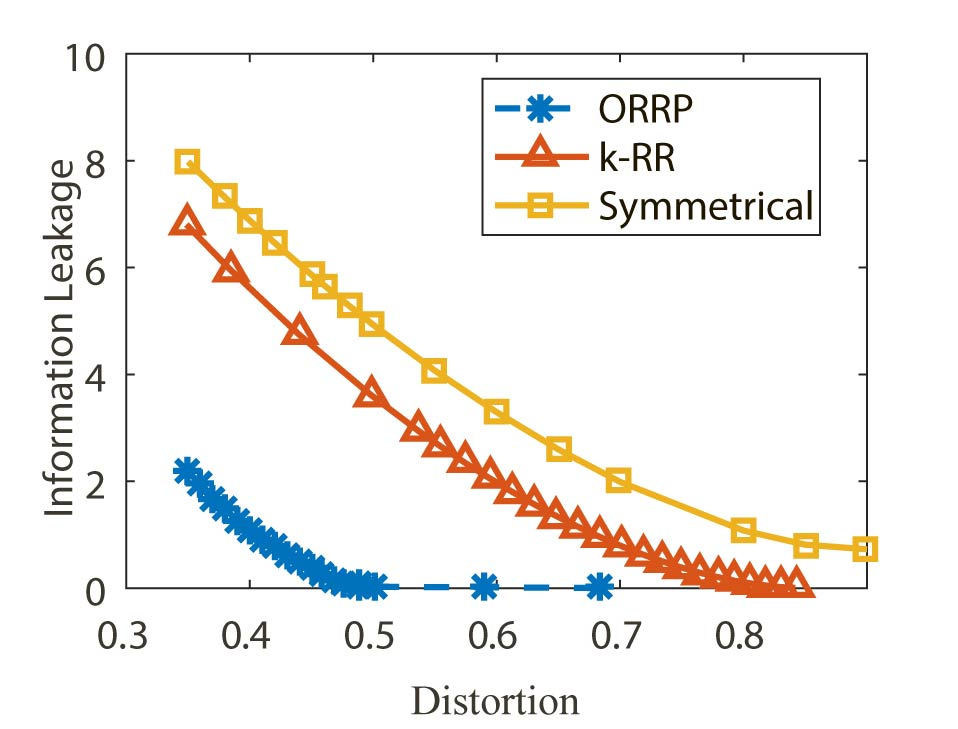
\includegraphics[width=170pt,height=130pt]{./figures/chapter06/MI_ED_Adult.jpg}
%\caption{收敛门限与互信息隐私泄露量}
%\end{minipage}
%\begin{minipage}[t]{6cm}
%\centering
%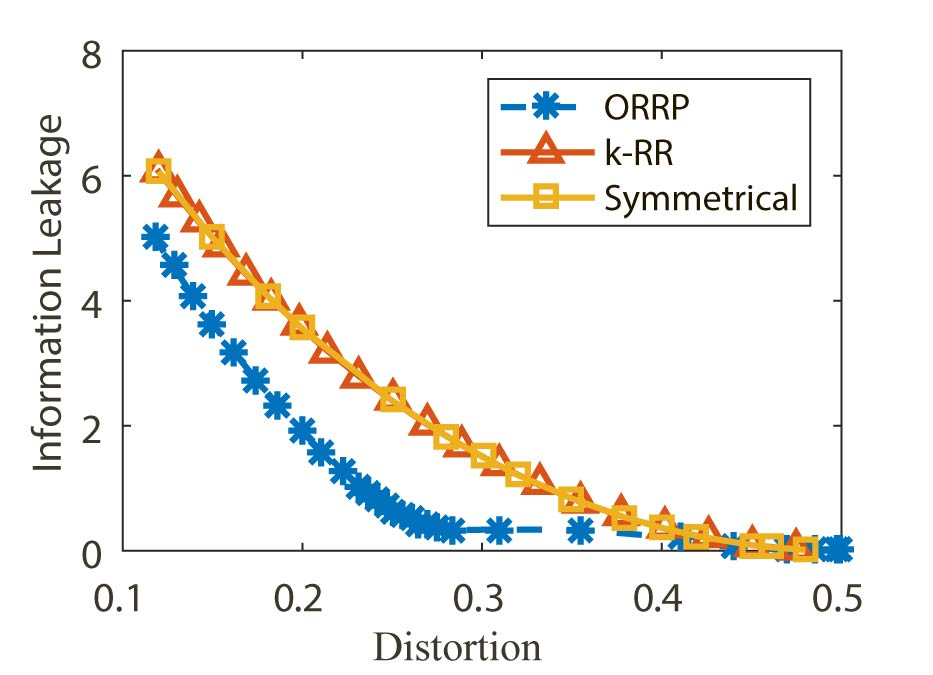
\includegraphics[width=170pt,height=130pt]{./figures/chapter06/MI_ED_NLTCS.jpg}
%\caption{收敛门限与期望失真度}
%\end{minipage}
%\begin{minipage}[t]{6cm}
%\centering
%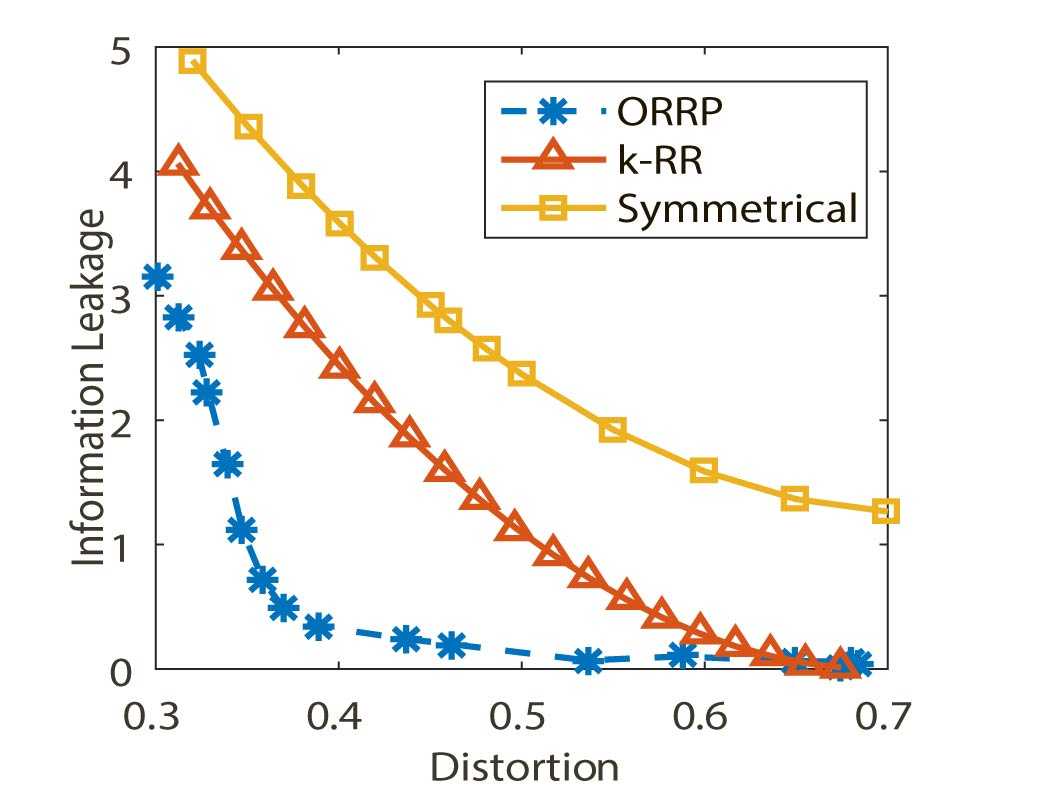
\includegraphics[width=170pt,height=130pt]{./figures/chapter06/MI_ED_CRX.jpg}
%\caption{收敛门限与期望失真度}
%\end{minipage}
%\end{figure}


其次,Wang等\cite{wang2019collecting}提出的分段机制(PM)、混合机制(HM)是目前对多维混合数值型和类别型属性处理的先进LDP机制。本节中与PM机制进行比较,提供主要的比较和分析结果。首先,Wang等的方法在处理多维属性时,先将属性分为数值型和类别型两类,使用不同的隐私机制进行扰动处理。对于数值型数据,应用分段机制(PM)随机扰动,而对于类别型数据,则使用存在的任意单一类别型隐私机制,如OUE。对比与PM,本章中提出的ORRP方法提供了一个统一的数据处理,这得益于单属性最优化模型计算概率分布函数。其次,本章中提出的方法可以对属性级保护设置不同的隐私参数,这是缩放优化模型约束参数具体的优势。最后,PM机制对于多维数据随机扰动处理的一个关键步骤是计算一个整数$k$,表示元组中随机扰动的属性数,然后在属性集中均匀的抽样$k$个属性随机扰动真实的元组。其中的$k$依据公式$k=\max\left\{1,\min\left\{d,\lfloor\frac{\epsilon}{2.5}\rfloor\right\}\right\}$计算,其依赖于$\epsilon$的具体取值,因此则有

\begin{equation}\label{eq:pm}
	k=\left\{
	\begin{array}{lcl}
		1, & & {0 < \epsilon <5},\\
		{\{2,\cdots,d-1\}}, & & {5 \leq \epsilon <2.5d},\\
		d, & & {2.5d \leq \epsilon}.
	\end{array}\right.
\end{equation}

上述公式\ref{eq:pm}表示了可能存在的$3$种情况,即是,随机的扰动元组中单个属性、部分的属性和所有全部的属性。首先,如果$\epsilon$值很小并且$d$的值足够大,则PM机制随机的保护整个元组中的单个属性。其次,参考随机响应整个元组的方法\cite{andres2013geo},PM机制响应整个元组当且仅当有一个足够大的隐私参数($\epsilon>2.5d$)。在这样的情况下,PM机制将提供较弱的隐私保护。最后,当$5\leq \epsilon \leq 2.5d$时,其对整个元组中的部分属性提供隐私保护。然而,本章中提出的方法可以提供元组全部属性的保护,即使有一个较小的隐私参数。而且,可以通过调整不同属性优化问题的$\lambda$取值,获得属性级的最优隐私机制。接下来,讨论所提出的隐私机制在实践中的优势。

通过实现PM机制的伪代码并在真实数据集上执行,首先比较提出的机制与PM机制对于一维数值型数据(如表~\ref{tab:origin}~Adult数据集中的Age属性)的处理。对于Wang 等的PM 机制,遵循提出的三个步骤,将原数据归一化到$[-1,1]$的区间,得到扰动的值。例如,当$\epsilon=0.5$时,计算$C=8.042$,则PM机制扰动输出区间$[-8.042,8.042]$区间的一个扰动值,然后发送$r$与扰动值的一个乘积给数据收集者。对比这个过程,给出以下的讨论和分析。PM机制输出的扰动值$v' \in [-r*C,r*C]$,这个随机扰动过程为了维持高的数据统计精确度牺牲了数据真实的语义。例如,Age通常被认为是一个数值型数据,其值来源于$0$到一个合适的正整数。然而,PM机制的扰动输出结果可能出现负值和一个充分大的单精度数值,这将很难适应这种语义的要求。为了保持数据的完整性并体现语义的约束,一些方法(如基于门限的单侧过滤法)可能会被使用去克服这个问题。此外,在一些基于数据的服务中报告的数据应该属于一个离散的集合。例如,基于位置的服务应用中通常考虑用户的位置由经、纬度坐标组成。对于这样的数值数据,PM机制产生的输出可能超出原始的边界,可能导致无效的数据效用。然而,信息论的方法可以有效解决该问题,通过划分区域到一些认真选择的网格\cite{zhang2019online},保证了报告的数据落在一个特定的离散集合\cite{oya2017back}。对比PM机制,所提出的方法报告扰动数据使用其原始数据域,对于语义完整性的支撑较好。

其次,对于~$d$~维元组的随机扰动处理,PM机制随机、均匀的从$d$-维元组中扰动$k$个属性。当元组中包含多维类别型数值时(如NLTCS数据集中包含``0''和``1''),PM机制将退化为已存在的针对类别型属性的扰动方案。这样的问题可以较好的使用提出的ORRP方案解决,这得益于汉明失真函数的优势。接下来,使用{\em NLTCS}作为实例说明本章的观点。当$0<\epsilon < 5$时,PM机制仅扰动$16$个属性中随机抽样的$1$个属性,获得单一选择属性的扰动结果。如此以来,有关个人的其它属性信息相当于完全的裸露。而且,没有考虑数据先验分布的影响。如果是非均匀的分布,一个消息灵通的敌手可以有较高的置信推断私密信息。然而,本章中提出的方法可以实现全数据元组的隐私保护。进一步,当且仅当$\epsilon \geq 40$时,PM机制随机的响应整个元组,并且它的性能依赖于选择的单一属性的扰动机制。如果将最优的二元编码(OUE)\cite{wang2017locally}替换为$k$-RR或对称机制,则有以下的比较结果。

\begin{figure*}[htbp]
	\centering
	%\vspace{-0.35cm}
%	\subfigtopskip=2pt %设置子图与上面正文或别的内容的距离
%	\subfigbottomskip=2pt %设置第二行子图与第一行子图的距离,即下面的头与上面的脚的距离
%	\subfigcapskip=-5pt %设置子图与子标题之间的距离
	\subfigure[Adult数据集]{
		\begin{minipage}[t]{5.2cm}
			\centering
			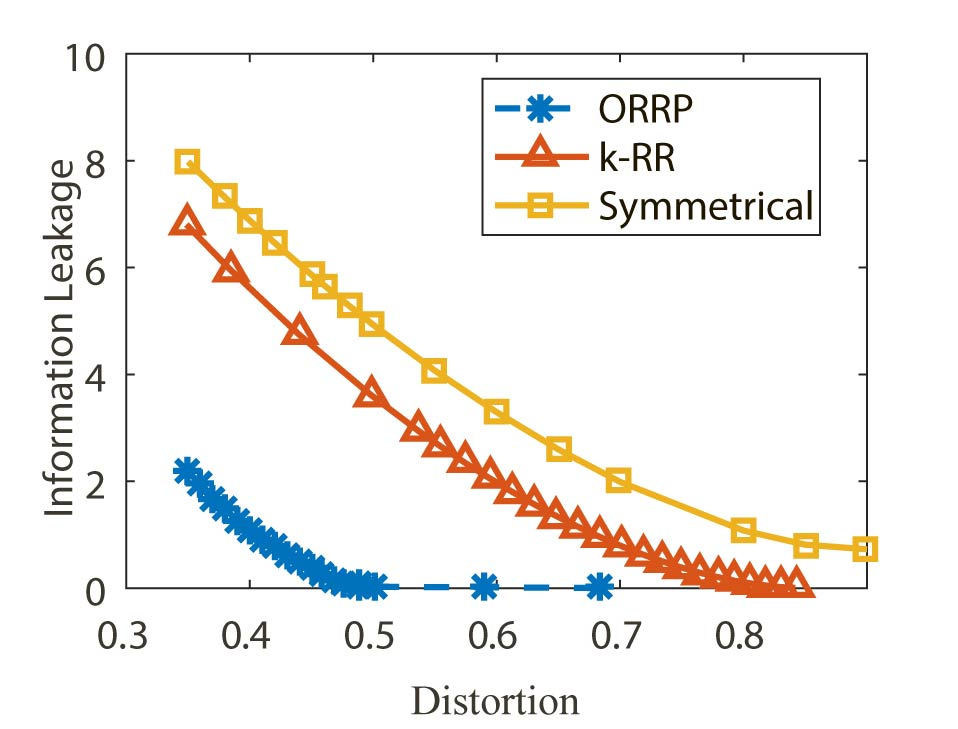
\epsfig{file=./figures/chapter06/MI_ED_Adult.jpg, width=165pt,height=130pt}
			\label{Fig:MI_ED_Adult}
		\end{minipage}%
	}%
	\subfigure[NLTCS数据集]{
		\begin{minipage}[t]{5.2cm}
			\centering
			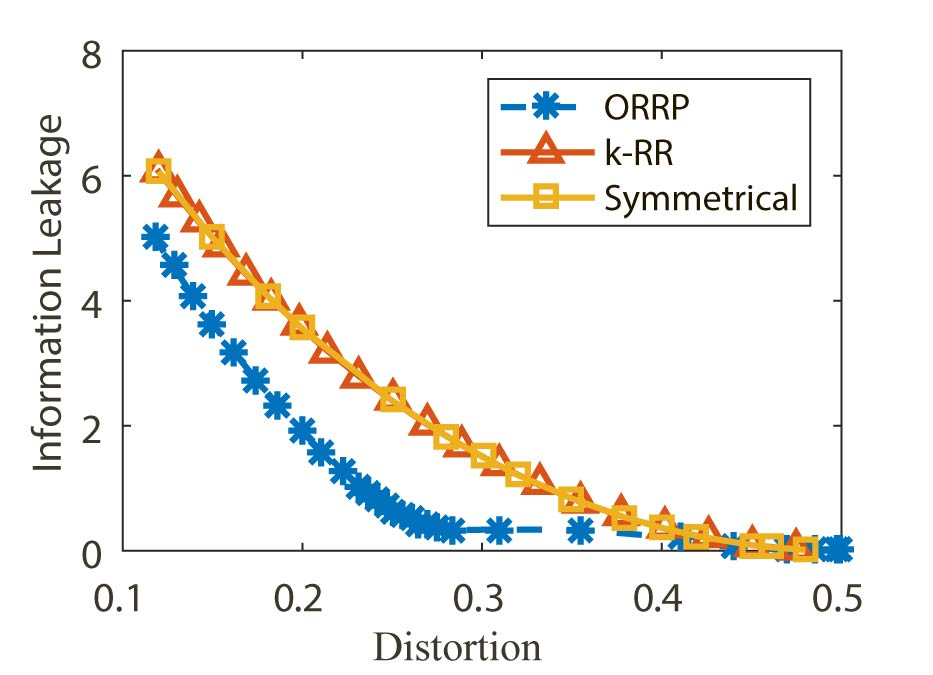
\epsfig{file=./figures/chapter06/MI_ED_NLTCS.jpg, width=165pt,height=130pt}
			\label{Fig:MI_ED_NLTCS}
		\end{minipage}%
	}%
	\subfigure[Credit Approval数据集]{
		\begin{minipage}[t]{5.2cm}
			\centering
			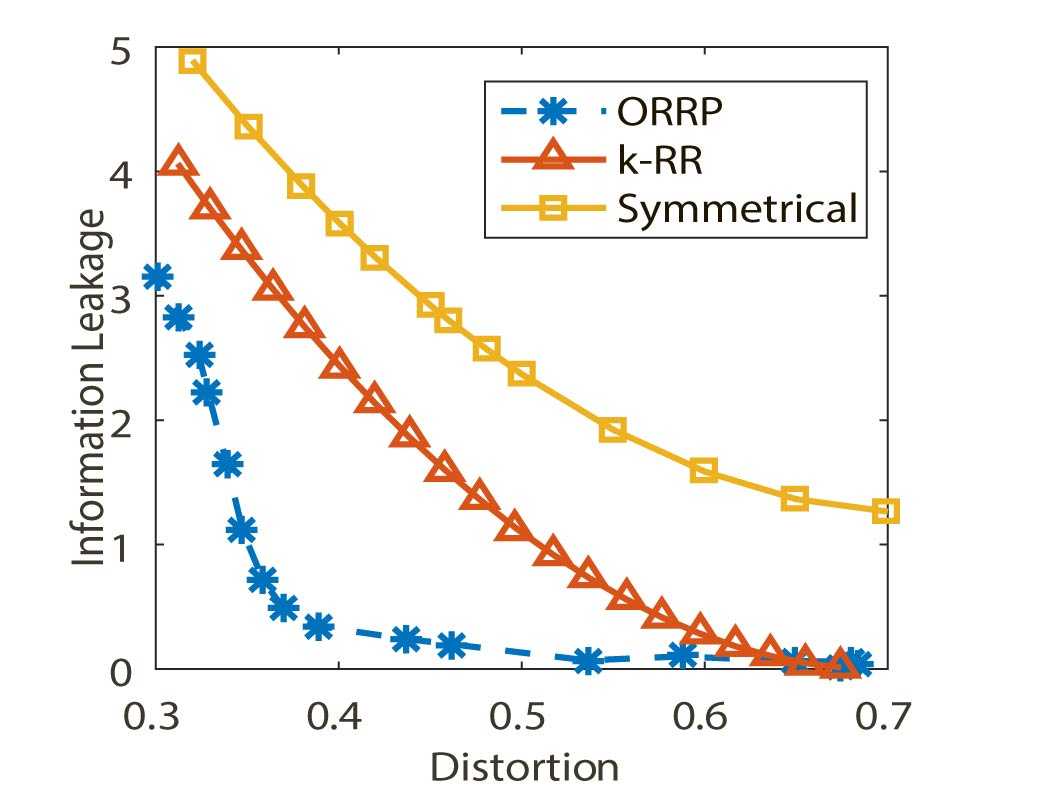
\epsfig{file=./figures/chapter06/MI_ED_CRX.jpg, width=165pt,height=130pt}
			\label{Fig:MI_ED_CRX}
		\end{minipage}
	}%
	\centering
	\caption{不同隐私机制的信息泄露和失真对比}
	\label{Fig:5}
\end{figure*}

除了上面提到的,以下在三个真实的数据集上设置不同的参数与另外两个存在的机制进行比较。在信息论方法的隐私保护研究工作中,注意到所提出隐私机制的性能通常使用信息泄露和失真进行分析(如文献\mycite{kalantari2018robust,zhang2019online,sarwate2014a})。为了有一个公平的比较,本章从信息泄露和失真的角度给出比较结果分析。对于本章中提出的隐私机制,设置$\lambda$从$0.1$增加到$2.0$进行实验,并在图~\ref{Fig:5}中显示出与$k$-RR和对称机制的对比结果。具体来说,图~\ref{Fig:MI_ED_Adult}显示了$T=10^{-5}$时Adult数据集平均失真与互信息量化的信息泄露之间的关系。从图中可以得知,本章所提出的ORRP 机制在保持相同的失真时具有较少的信息泄露。同样的,$T=10^{-3}$时的图~\ref{Fig:MI_ED_NLTCS}和$T=10^{-5}$时的图~\ref{Fig:MI_ED_CRX}分别使用NLTCS和Credit Approval数据集说明了一个相似的结果。特别的,对于``0'',``1''类型数据,$k$-RR与对称机制在图~\ref{Fig:MI_ED_NLTCS}中具有相同的结果。综合分析,图~\ref{Fig:5}中的三组实验结果都证实了所提出的ORRP机制在保证同等级信息泄露的同时,具有较少的数据质量损失。实践中,提出的ORRP机制提供有区别的属性级保护依赖于单属性优化模型中决定最优概率密度函数的参数选取。由此,有必要研究参数对隐私机制的影响。接下来,分析参数$\lambda$和$T$的影响,并给出实际选取时应该考虑的因素。


\subsection{参数$\lambda$影响}\label{sec:Impactlambda}

对于单属性的优化模型使用拉格朗日乘子法求解,并进一步以B-A算法为基础设计ORRP,拉格朗日乘子$\lambda$影响提出ORRP机制的最优概率密度函数。特别地,文献\mycite{oya2017back}中证明上述方式获得的隐私机制在位置隐私保护中提供$\epsilon_j=2\lambda$-geo-indistinguishability。据此,参数$\lambda$对隐私机制的不可区分等级具有直接的影响,也就是,本章中提出的ORRP的隐私等级与拉格朗日乘子函数相关。在此不再给予过多的强调,因为不可区分性比较直观。接下来,本小节中使用信息论的度量方法研究参数的影响,将其划分为以下三个方面。


(1) {\em 参数$\lambda$对信息泄露的影响}。通过选定不同的~$\lambda$~和~$T$~参数,在三个不同的数据集上进行实验,以实验结果分析不同的~$\lambda$~ 取值对互信息隐私泄露的影响。由于数据集数据分布的特征,~$\lambda$~和~$T$~的取值选择有所不同,但能反映出整体的趋势。固定~$T$~的取值时,图~\ref{Fig:6} 中的一组实验结果表明信息泄露量随着~$\lambda$~的增长而增加,这样的增长趋势可以被解释为随着~$\lambda$~的增加,ORRP机制对元组提供的隐私保护强度整体减弱。具体地说,当$0.1 \leq \lambda \leq 2.0$时,图~\ref{Fig:MI_Adult}中显示了Adult数据集上三组不同~$T$~取值的结果,图中曲线表示出了信息泄露和~$\lambda$~的变化关系。相似的,当$0.1 \leq \lambda \leq 2.0$时,图~\ref{Fig:MI_Nlcts}展示了在3个不同$T$取值时NLTCS 数据集的实验结果,互信息隐私信息泄露量随$\lambda$同样具有增长的趋势。进一步,对于$0.1 \leq \lambda \leq 1.0$,Credit Approval 数据集在不同~$T$~值的实验结果和前者具有相同的趋势。
\begin{figure*}[htbp]
\centering
\subfigure[Adult数据集]{
\begin{minipage}[t]{5.2cm}
\centering
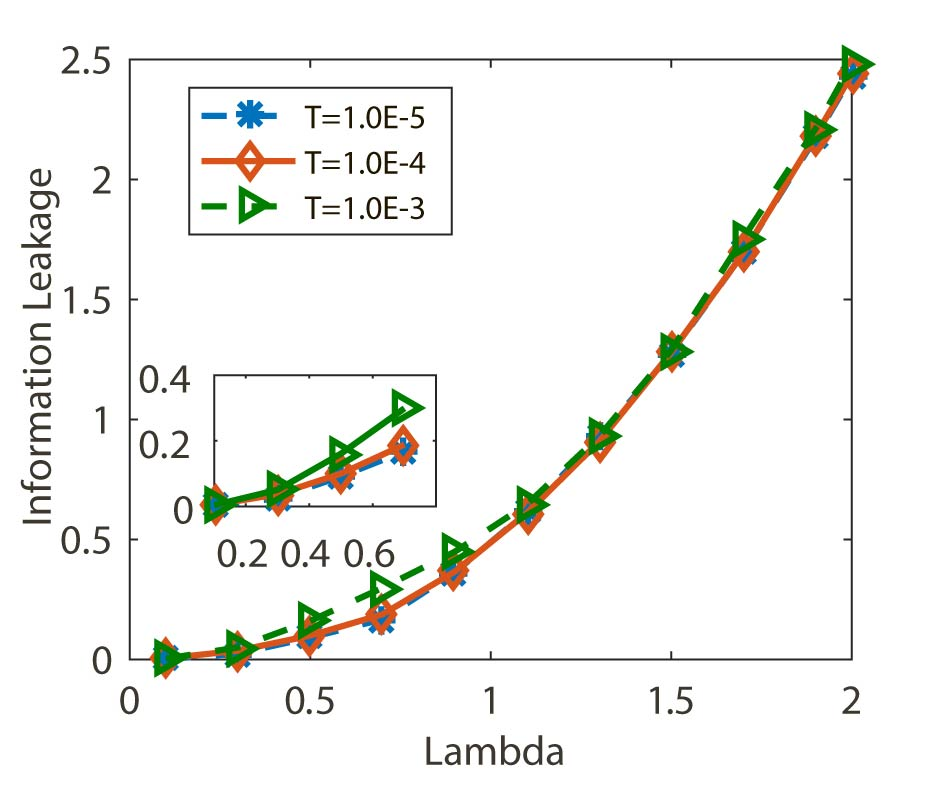
\epsfig{file=./figures/chapter06/MI_lambda_adult.jpg, width=165pt,height=130pt}
%\caption{fig1}
\label{Fig:MI_Adult}
\end{minipage}%
}%
\subfigure[NLTCS数据集]{
\begin{minipage}[t]{5.2cm}
\centering
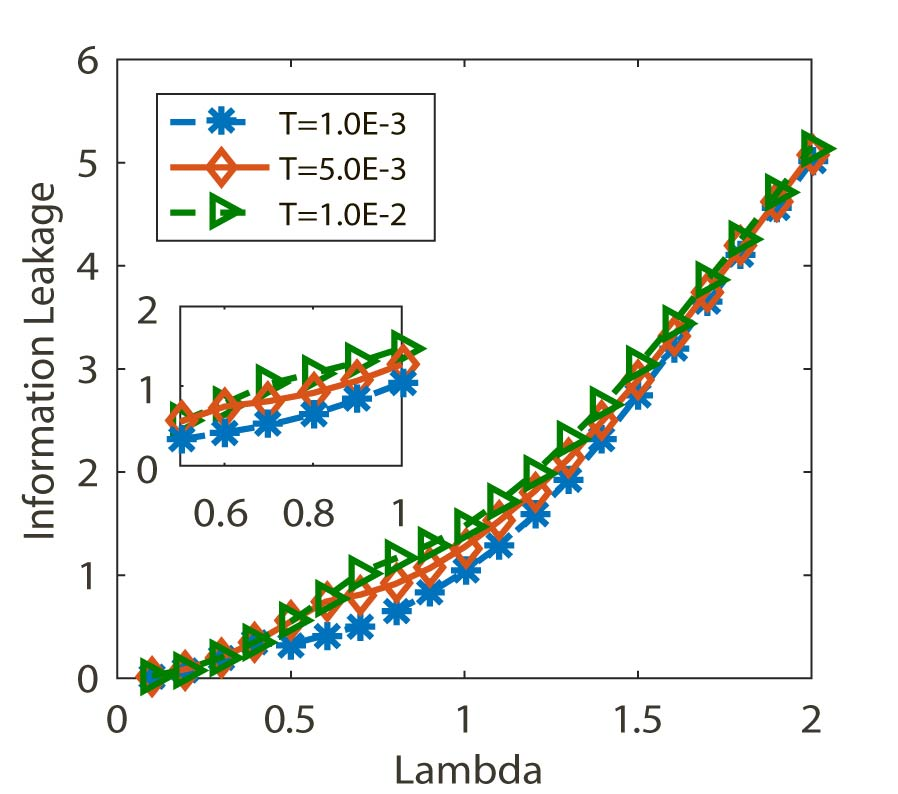
\epsfig{file=./figures/chapter06/MI_Lambda_nlcts.jpg, width=165pt,height=130pt}
%\caption{fig2}
\label{Fig:MI_Nlcts}
\end{minipage}%
}%
\subfigure[Credit Approval数据集]{
\begin{minipage}[t]{5.2cm}
\centering
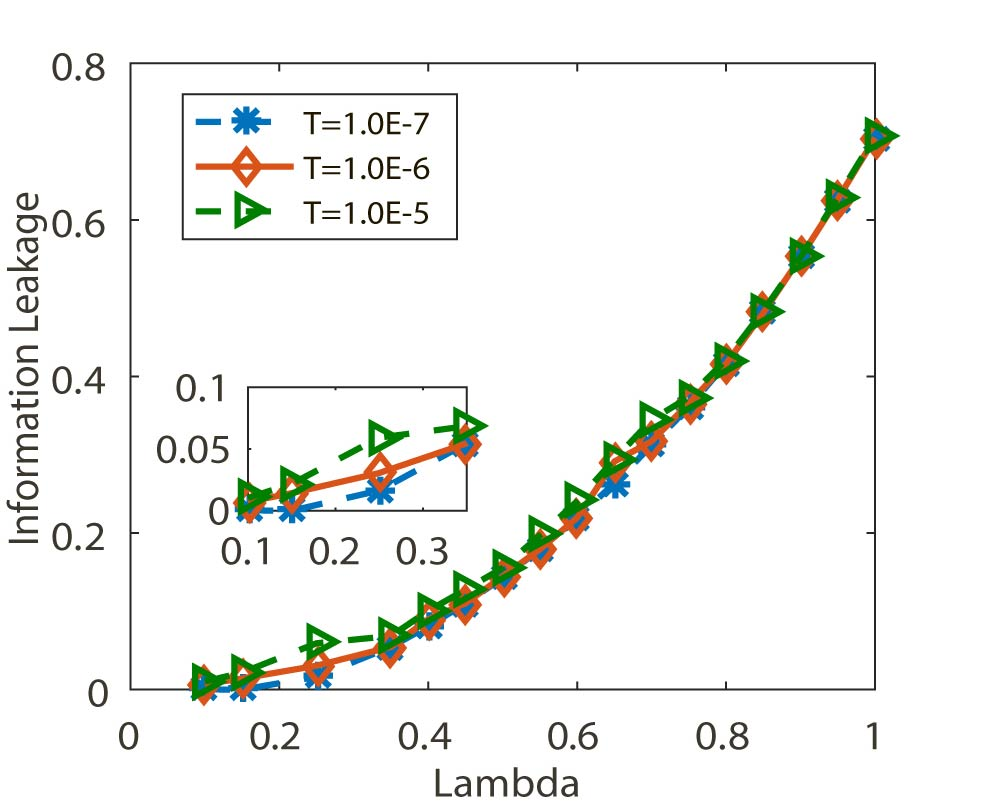
\epsfig{file=./figures/chapter06/MI_Lambda_crx.jpg, width=165pt,height=130pt}
%\caption{fig2}
\label{Fig:MI_Crx}
\end{minipage}
}%
\vspace{-0.3cm}
\centering
\caption{ORRP方案隐私信息泄露的参数影响}
\label{Fig:6}
\end{figure*}
\vspace{-0.1cm}

(2) {\em 参数$\lambda$对数据质量损失的影响}。为了能和隐私信息泄露的变化图~\ref{Fig:6}对比说明问题,在此,对$\lambda$和$T$选定和上述相同的取值,图~\ref{Fig:7}显示了在三个数据集上执行的实验结果。总体上,基于失真量化的数据质量损失随着$\lambda$的增加而减少,这个结论可以被解释为ORRP机制提供的隐私保护强度随着$\lambda$增加而减弱,从而导致具有较少的失真,数据质量提升。对比图~\ref{Fig:6}和图~\ref{Fig:7}分析,隐私信息泄露与失真变化具有相关的趋势,从通信的角度解释为信宿与信源消息完全不相关时,失真程度最大而信源不确定度无减少。具体数据集的实验,图~\ref{Fig:ED_Adult}显示了Adult数据集结果,随着$\lambda$增加,失真表现出了减少的趋势。对于$3$个不同的$T$值,都有同样的趋势。此外,图~\ref{Fig:ED_Nlcts}和图~\ref{Fig:ED_Crx}均证实了一个同样的结论。在这个过程中的一些关键影响点在\ref{sec:impactofT}小节中介绍。
\begin{figure*}[htbp]
\centering
\subfigure[Adult数据集]{
\begin{minipage}[t]{5.2cm}
\centering
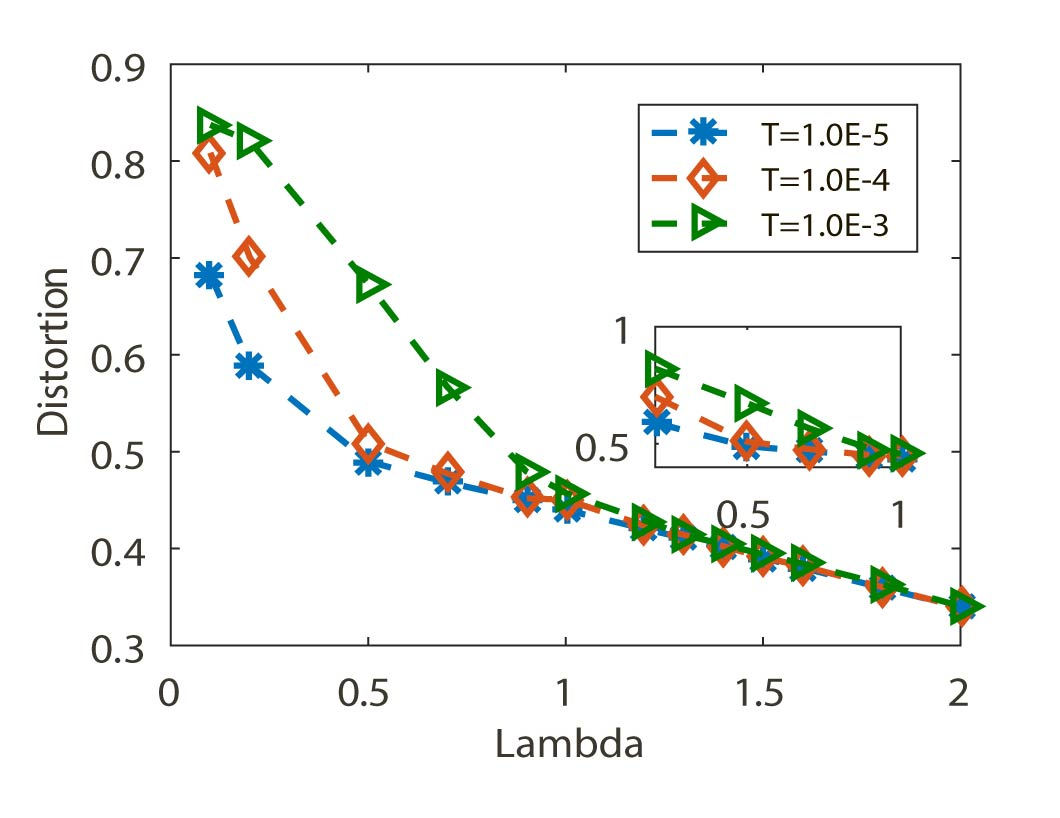
\epsfig{file=./figures/chapter06/ED_lambda_adult.jpg, width=165pt,height=130pt}
%\caption{fig1}
\label{Fig:ED_Adult}
\end{minipage}%
}%
\subfigure[NLTCS数据集]{
\begin{minipage}[t]{5.2cm}
\centering
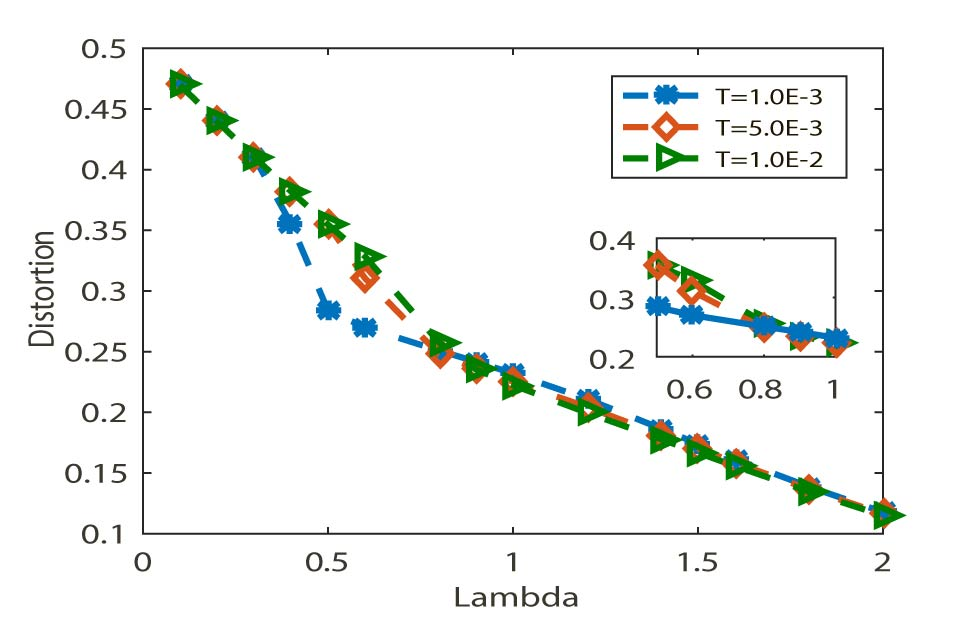
\epsfig{file=./figures/chapter06/ED_lambda_nltcs.jpg, width=165pt,height=130pt}
%\caption{fig2}
\label{Fig:ED_Nlcts}
\end{minipage}%
}%
\subfigure[Credit Approval数据集]{
\begin{minipage}[t]{5.2cm}
\centering
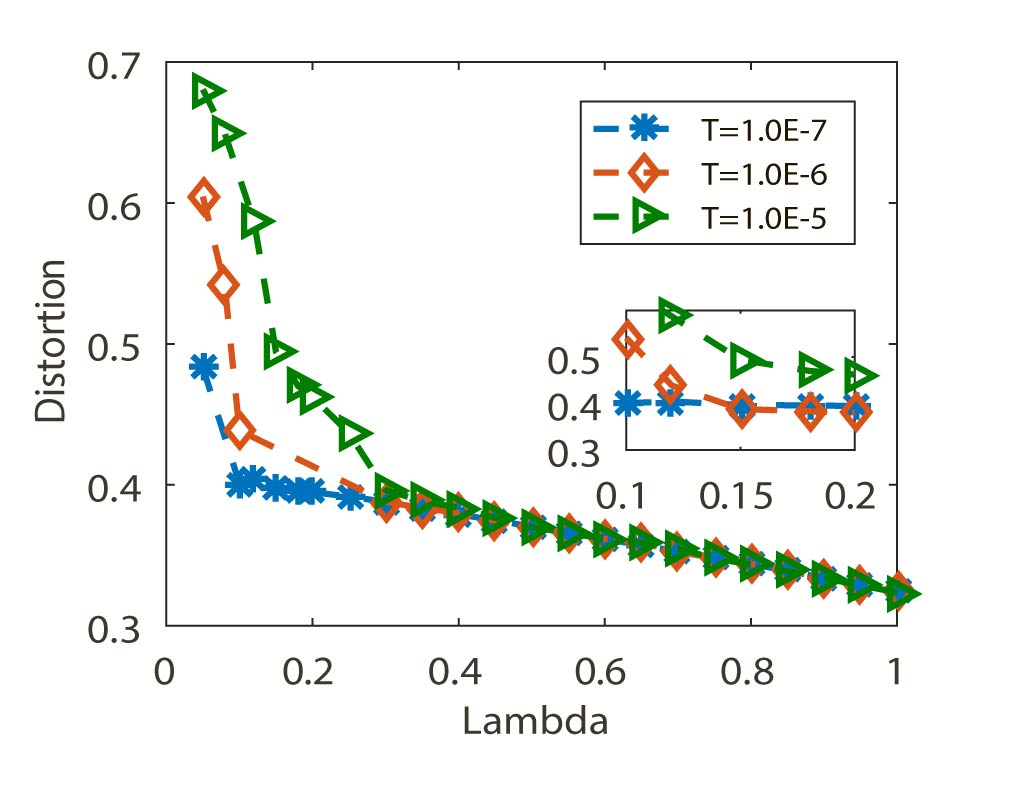
\epsfig{file=./figures/chapter06/ED_lambda_crx.jpg, width=165pt,height=130pt}
%\caption{fig2}
\label{Fig:ED_Crx}
\end{minipage}
}%
\vspace{-0.3cm}
\centering
\caption{ORRP方案数据质量损失的参数影响}
\label{Fig:7}
\end{figure*}
%图
\vspace{-0.1cm}

(3) {\em 参数$\lambda$对属性相关度损失的影响}。实验中针对$3$个数据集选择不同的$\lambda$和$T$,通过结构信息测量比较由于隐私保护机制随机扰动引起的报告元组和原始元组之间的结构信息量变化,用于量化相关度的损失。为了克服ORRP算法\ref{alg:ORRP}的随机性,对于每一组选定的$\lambda$和$T$的组合重复执行$5$次实验。三个不同数据集的实验结果如表~\ref{Tab:impactofNSE}中数据。首先,选择$\lambda=0.2,0.6$和$T=0.01,0.005$,利用算法\ref{alg:ORRP}有序得到报告的元组。进一步,使用$\phi_{c}=0.02$量化结构信息。随后,比较结构信息的改变量。基于表~\ref{Tab:impactofNSE}可知,当固定$T$时,随着$\lambda$的增加,结构信息有较小的损失。具体的,固定$T=0.01$时,Adult原始的结构信息是$3.17$,$\lambda=0.6$的隐私机制随机扰动后结构信息是$3.141$,大于$\lambda=0.2$时的$3.126$。也就是,信息泄露随着$\lambda$增加而增加,而数据失真在减少。由此,在一定程度上,相关度损失随$\lambda$增加而减少。此外的两组实验,也有相似的结果。例如,NLTCS的实验结果,$\lambda = 0.6,T=0.01$时的$3.986$大于$\lambda = 0.4,T=0.01$时的$3.858$,对比原始的$4.0$表明前者具有较小的相关度损失。然而,$\lambda$和$T$的共同作用会产生一定的影响,对于$T$的影响在\ref{sec:impactofT}小节中给出具体的分析。

\begin{table}[htbp]
	\caption{说明~$\lambda$~和~$T$~对相关度损失的影响}
	\footnotesize
	\centering \label{Tab:impactofNSE}
	\begin{tabular}{p{0.15\textwidth}p{0.18\textwidth}p{0.18\textwidth}p{0.18\textwidth}p{0.18\textwidth}}
		\toprule
		&\multicolumn{3}{c}{设置$\phi_{c}=0.02$评估结构信息的影响(原始的$3.17$)}& \\
		{\em Adult}&$\lambda=0.6,T=1.0E-2$&$\lambda=0.6,T=5.0E-3$&$\lambda=0.2,T=1.0E-2$&$\lambda=0.2,T=5.0E-3$ \\
		\midrule
		&$3.141$    &$3.143$    &$3.126$    &$3.12$\\
		\midrule
		&\multicolumn{3}{c}{设置参数~$\phi_{c}=0.02$ (原始的$4.0$)}& \\
		{\em NLTCS}&$\lambda=0.6,T=1.0E-2$&$\lambda=0.6,T=1.0E-3$&$\lambda=0.4,T=1.0E-2$&$\lambda=0.4,T=1.0E-3$ \\
		\midrule
		&$3.986$    &$3.672$    &$3.858$ &$3.885$\\
		\midrule
		&\multicolumn{3}{c}{设置参数~$\phi_{c}=0.02$ (原始的$3.46$)}& \\
		{\em Credit Approval}&$\lambda=0.6,T=1.0E-2$&$\lambda=0.6,T=1.0E-3$ &$\lambda=0.5,T=1.0E-2$&$\lambda=0.5,T=1.0E-3$\\
		\midrule
		&$3.4538$ &$3.4554$     &$3.4558$     &$3.4561$     \\
		\bottomrule
	\end{tabular}
\end{table}

事实上,在实际中可以通过缩放针对不同属性计算最优条件分布时的$\lambda$值获得不同的保护级别。例如,为每个属性$X_j$的优化模型求解中设置不同的$\lambda$(回顾\ref{subsec:MI_optimal_mechanism}小节),可以得到不同级别的隐私保护机制$Q_j$。进一步,基于定理\ref{theorem:chapter06_sequence} 保证ORRP机制的组合性能。特别的,一个恰当选择的$\lambda$可以表达用户的隐私偏好,控制隐私信息泄露和数据失真在一个可接受、可容忍的范围内。

\subsection{参数$T$影响}\label{sec:impactofT}
本章中所提出的ORRP机制是单属性隐私最优机制的组合$\{Q_j\}_{j=1}^{d}$,对于$Q_j$,$T$是收敛门限,控制交替最小化算法\ref{alg:B-A}的轮数,所以,$T$对最优的输出概率分布有一个直接的影响。为了给予分析$T$的影响,在上述\ref{sec:Impactlambda}小节中设置不同的$T$进行实验。首先,基于图~\ref{Fig:6}分析$T$对隐私信息泄露的影响,从图中看出,较小的$T$拥有较大的信息泄露。但是,当$\lambda$超过一个关键的值时,$T$的影响变得非常微弱。在图~\ref{Fig:MI_Adult}中,对于 $T=0.00001, 0.0001, 0.001$ 和 $\lambda=1.5$时,信息泄露量分别是$1.2747, 1.2798, 1.2882$ 。当$\lambda>1.5$时,$T$对信息泄露的影响变得非常微弱。除此之外的另两组数据集上的实验拥有一个相似的结果。图~ \ref{Fig:MI_Nlcts} 显示了$T=0.001,0.005,0.01$的结果,当$\lambda>1.8$时,信息泄露仅有轻微的变化。从$\lambda >0.75$时,图~\ref{Fig:MI_Crx}呈现了相似的变化。其次,从图~\ref{Fig:7}中可以看出$T$对数据质量损失的影响。当$\lambda$值较小时,随着$T$的增加,失真有一个较大的变化幅度。基于图~~\ref{Fig:6}和图~\ref{Fig:7}分析,固定$\lambda$取值时,较小的$T$可以减少信息泄露和失真,这可以被解释为一个较小的值使得互信息收敛到临近值,得到的最优分布和初始的均匀分布差别较大。当$\lambda >1.5$时,Adult数据集的实验结果图~\ref{Fig:MI_Adult}表明对于不同的$T$具有轻微的变化。此外的两组实验图~\ref{Fig:MI_Nlcts} 和图~\ref{Fig:ED_Crx}证实了$T$的影响。

此外,通过设置合适的参数($\phi_{c}=0.02$),研究了$T$对属性相关度损失的影响。从表~\ref{Tab:impactofNSE}中的实验数据看出当减少$T$的值时,结构信息的变化量变大,即是,当$T$减少时则会产生一个较大的相关度损失。但是,这个作用非常轻微并且受到不同的$\lambda$影响,图~\ref{Fig:6} 中也有相同体现。

基于实验结果,上述分析了参数$T$的影响。一个很自然的问题是:对于隐私机制设计,如何选择一个恰当的$T$实现隐私泄露与数据质量损失的权衡?直观地说,设置一个合理的$T$应该考虑特殊的先验分布和不同的应用需求。此外,$T$还与最优化模型求解的计算时间有关,$T$的增加会降低计算时间。在实际中,$T$应该由隐私容忍度和数据质量决定。如果$T$对隐私泄露影响轻微的一些应用,可以在隐私容忍度条件下适当选择一个稍大的$T$。

\section{本章小结}\label{sec:chapter05-conclusion}
本章针对差分隐私数据收集中多维数据处理的隐私脆弱性和有效性问题,为了权衡隐私泄露与数据质量损失,利用信息论的方法提出了有序随机响应扰动(ORRP)方案。首先,对于元组的多维属性使用分治策略思想分解元组属性,构建本地扰动的独立并联信道模型。其次,针对单属性分量的隐私保护问题,基于信息论的度量方法形式化数据质量损失约束前提下最小化隐私信息泄露的最优化模型,用于计算最优概率密度函数(PDF)。然后,以B-A为基本构建模块设计ORRP,利用上述PDF实现有序随机响应,并给出算法描述。最后,给出理论分析和真实数据集上的实验结果。
